\documentclass[
        a4paper,     % Format A4
        titlepage,   % mit Titelseite
        twoside,     % zweiseitig
        parskip      % mit Durchschuss
                                 % (= Abstand zwischen Absätzen, statt Einrückung)
        ]{scrartcl} %{} % KOMA-Script Grundklasse     texdoc scrguide

\usepackage[american]{babel}             
\usepackage[T1]{fontenc}          % Schriftkodierung mit Umlauten
\usepackage{textcomp,amsmath}     % Mathezeichen etc.
\usepackage{graphicx}             % Graphiken einbinden

\usepackage{acro}                 % List of abbriviations 
\usepackage[toc,page]{appendix}   % Appendixes
\usepackage{listings}             % Code Blocks
\usepackage{color}

\usepackage{microtype} 			  % enable margin kerning
\usepackage{booktabs}		      % table stuff, like toprule

% Table styles % 
\setlength{\tabcolsep}{18pt}
\renewcommand{\arraystretch}{1.5}

% Code Listing Styles
\definecolor{backcolour}{rgb}{0.95,0.95,0.92}
\lstdefinestyle{mystyle}{
    backgroundcolor=\color{backcolour},   
    captionpos=b,
    breaklines=true,
    basicstyle=\footnotesize,
    numbers=left,                    
    numbersep=5pt,  
}
\lstset{style=mystyle}

% probably a good idea for the nomenclature entries:
\acsetup{first-style=short}

% bibtex
\usepackage{url}
\bibliographystyle{plaindin}      % BibTeX Styles nach Norm DIN 1505

\titlehead{

\includegraphics{hpi_logo_cmyk_wb_sl2}
} \subject{Master Thesis}
\title{Language Identification using Deep Convolutional Recurrent Neural Networks
\\ \bigskip 
\large{<Deutscher Titel bei englischer Arbeit> }}
\author{Tom Herold\\{\small{\url{tom.herold@student.hpi.uni-potsdam.de}}}}
\date{XX.02.2016}
\publishers{
Supverisors \\ Prof. Dr. Christoph Meinel \\ Dr. Haojin Yang \\
\bigskip 
Internet-Technologies and Systems \\
Hasso Plattner Institute \\
University of Potsdam, Germany 
}


\pagestyle{headings}    % Seitenstil mit Kapitelüberschriften in der Kopfzeile

% class `abbrev': abbreviations:
\DeclareAcronym{ann}{
  short = ANN,
  long = artificial neural network,
  class = abbrev
}
\DeclareAcronym{dnn}{
  short = DNN,
  long = deep neural network,
  class = abbrev
}
\DeclareAcronym{rnn}{
  short = RNN,
  long = recurrent neural network,
  class = abbrev
}
\DeclareAcronym{cnn}{
  short = CNN,
  long = convolutional neural network,
  class = abbrev
}
\DeclareAcronym{lstm}{
  short = LSTM,
  long = long short-term memory,
  class = abbrev
}
\DeclareAcronym{eer}{
  short = EER,
  long = equal error rate,
  class = abbrev
}
\DeclareAcronym{far}{
  short = FAR,
  long = false accept rate,
  class = abbrev
}
\DeclareAcronym{fc}{
  short = FC,
  long = fully connected,
  class = abbrev
}
\DeclareAcronym{frr}{
  short = FRR,
  long = false reject rate,
  class = abbrev
}
\DeclareAcronym{gpu}{
  short = GPU,
  long = graphics processing unit,
  class = abbrev
}
\DeclareAcronym{mlp}{
  short = MLP,
  long = multilayer perceptron,
  class = abbrev
}
\DeclareAcronym{mse}{
  short = MSE,
  long = mean squared error,
  class = abbrev
}
\DeclareAcronym{nist}{
  short = NIST,
  long = National Institute of Standards and Technology,
  class = abbrev
}
\DeclareAcronym{pca}{
  short = PCA,
  long = principal component analysis,
  class = abbrev
}
\DeclareAcronym{pdf}{
  short = PDF,
  long = probability density function,
  class = abbrev
}
\DeclareAcronym{relu}{
  short = ReLU,
  long = Rectified Linear Unit,
  class = abbrev
}
\DeclareAcronym{roc}{
  short = ROC,
  long = receiver operating characteristic,
  class = abbrev
}
\DeclareAcronym{sgd}{
  short = SGD,
  long = stochastic gradient descent,
  class = abbrev
}
\DeclareAcronym{svm}{
  short = SVM,
  long = support vector machine,
  class = abbrev
}
\DeclareAcronym{tar}{
  short = TAR,
  long = true accept rate,
  class = abbrev
}
\DeclareAcronym{lid}{
  short = LID,
  long = language identification,
  class = abbrev
}
\DeclareAcronym{tsne}{
  short = t-SNE,
  long = t-distributed stochastic neighbor embedding,
  class = abbrev
}



\begin{document}

    \maketitle    %  Titelseite erzeugen

    \cleardoublepage % neue Doppelseite

    \pagenumbering{roman}
    \section*{\LARGE Abstract}
With the increasing ubiquity of voice input systems to computers, users rely on robust speech recognition algorithms to process their intents. The first step and key component to automatic speech recognition is \emph{language detection}. Without automatic language detection, speech utterances cannot be parsed correctly and grammar rules cannot be applied, causing subsequent speech recognition steps to fail.

A second trend in computer science is the successful application of deep neural networks on a variety of problems. In this thesis, we present a hybrid neural network system using deep learning techniques for automatic language identification for speech audio samples. Specifically, we apply convolutional recurrent neural networks on human speech input and evaluate their robustness in different environments.

Convolutional neural networks have shown great promise within the computer vision research community. Therefore, we base our research on established model architectures such as the Inception network~\cite{szegedy2015going} and transfer our audio-based research task into the image processing domain. We study the effectiveness of spectrogram images as a valuable input feature and discuss additional audio representations and related work for speech processing systems.

Deep learning systems benefit greatly from the availability of large-scale datasets. We train our models on more than \num{1000}~hours of speech audio in six different languages: English, German, French, Spanish, Mandarin Chinese, and Russian. We collect and process this data from speeches and sessions from the European Parliament as well as from news channels such as the BBC hosted on YouTube.

Our best-performing convolutional recurrent neural network scores a top accuracy and F1~score of \SI{96}{\percent} on the news dataset. With this approach, we report a constant improvement over various baseline convolutional neural networks. We evaluate our models in diverse noisy scenarios with data augmented to include white noise, crackling noise, and background music and observe a decrease in accuracy by~\num{5}~percentage points (p.p.), \num{3}~p.p., \num{7}~p.p., respectively. On the smaller EU~dataset, we achieve an accuracy and F1~score of~\SI{98}{\percent}.

    \cleardoublepage
    \section*{\LARGE Zusammenfassung}
Computer mit Spracheingabemöglichkeiten sind immer häufiger anzutreffen. Deshalb sind Nutzer vermehrt auf verlässliche Spracherkennungsalgorithmen angewiesen. Dabei ist automatische Sprachidentifizierung der erste und wichtigste Schritt für die eigentliche Spracherkennung. Ohne automatische Sprachidentifizierung sind alle weiteren Erkennungsschritt nutzlos, da weder Sprachklänge richtig verarbeitet noch Grammatikregeln korrekt angewandt werden.

Ein zweiter aktueller Trend in der Informatik ist die erfolgreiche Anwendung von tiefen neuronalen Netzwerken für eine Vielzahl von Aufgabenstellungen. In dieser Arbeit wird ein hybrides, neuronales Netzwerkmodell zur automatischen Identifizierung unterschiedlicher Sprachen mithilfe von \emph{Deep-Learning}-Techniken vorgestellt. Im Speziellen werden mehrere Modelle mit \emph{Convolutional Recurrent Neural Networks} auf menschliche Spracheingaben angewandt und deren Robustheit in verschiedenen Geräuschumgebungen evaluiert.

\emph{Convolutional Neural Networks} haben innerhalb der automatischen Bilderkennungsforschung beachtliche Durchbrüche erzielt. Deshalb wird unsere audiobasierte Forschungsfrage in die Bildverarbeitungsdomäne eingebettet. Darüber hinaus basiert diese Arbeit auf deren etablierten Modellarchitekturen wie beispielsweise dem Inception Netzwerk~\cite{szegedy2015going}. Dabei wird die Effektivität von Spektrogrammbildern als zielführendes Eingabemedium analysiert. Zusätzlich werden weitere Audiorepräsentationen und weiterführende Publikationen vorgestellt.

Insbesondere die Verfügbarkeit von großen Datensätzen kommen Deep-Learning-Systemen zugute. Unsere Modelle werden auf mehr als \num{1000}~Stunden an Sprachaufnahmen in sechs verschiedenen Sprachen trainiert: Englisch, Deutsch, Französisch, Spanisch, Mandarin und Russisch. Die Datengrundlage bilden Reden und Sitzungen des Europäischen Parlaments sowie YouTube-Kanäle verschiedener Nachrichtensender wie dem BBC.

Unser leistungsfähigstes Convolutional Recurrent Neural Network erreicht eine Erkennungsgenauigkeit und ein F-Maß von~\SI{96}{\percent} auf dem Nachrichtendatensatz. Unser Ansatz stellt eine konstante Verbesserung gegenüber allen getesteten Convolutional Neural Networks dar. Die Modelle werden zusätzlich in verschiedenen Szenarien mit künstlich veränderten Daten evaluiert. Dabei fügen wir Störgeräusche wie Rauschen, Geknister und Hintergrundmusik zu den Daten hinzu und messen einen Genauigkeitsverlust von jeweils \num{5}~Prozentpunkten (PP), \num{3}~PP und \num{7}~PP gegenüber den Originaldaten. Auf dem kleineren EU-Datensatz erreichen wir eine Genauigkeit und ein F-Maß von~\SI{98}{\percent}.

    \cleardoublepage
    \section*{\LARGE Acknowledgments}
I would like to express my gratitude to my supervisors Prof. Dr. Christoph Meinel and Dr. Haojin Yang. I want to thank them for giving me the opportunity to research this interesting topic, as well as for their guidance and advice. I especially want to thank Dr. Yang for his insights, support, and inspiration regarding the deep learning techniques used in my masters thesis.
I would also like to thank my colleagues Georg Wiese, Christian Bartz, Tom Bocklich, Norman Rzepka, and Johannes Jasper for the many fruitful discussions about language identification and machine learning in general. I owe them a great deal of gratitude for supporting and encouraging me while working on this thesis.

Thank you.


    \cleardoublepage
    
    \tableofcontents
    \clearpage
    \printacronyms[include-classes=abbrev,name=Abbreviations]
    
    \ac{lstm}

    \pagenumbering{arabic}
    \section{Introduction}

% context
% identify problem
% minimal related work
% contributions → sehr explizit, nicht zu detailliert
% structure

Computers have become ubiquitous in our daily lives. Millions of people around the world use speech input to conveniently interact with their devices.
Speech input excels in certain situations, such as hands-free interaction, when driving, or as an efficient alternative to text input instead of typing on small screens.
In all these interaction scenarios, the first step to understanding users is to correctly identify the input language. In some settings, computers might well use metadata such as known locations or the system's default languages for this task. Yet often times, it is much preferred to infer a language directly from the speech input. This can be the case in countries with more than one official language or for multilingual users. 

In the same timeframe of this development, deep learning and artificial neural networks have become the state of the art for many pattern recognition problems. 
Deep convolutional networks have become the best-performing method for solving various computer vision tasks, such as image classification~\cite{russakovsky2015imagenet}, object detection~\cite{russakovsky2015imagenet, everingham2010pascal}, text detection~\cite{Yang2016SceneTextRegAR, jaderberg2014synthetic}, semantic segmentation~\cite{dai2016instance, girshick2014rich}, object tracking~\cite{nam2016learning}, image retrieval~\cite{tolias2015particular}, and many others. 
The task of automatic language identification, however, was previously mainly done through classical machine learning algorithm approaches, which relied on domain-specific expert knowledge in the field of audio signal processing.



\subsection{Contributions}
In this thesis, we propose a novel system for language identification using deep learning techniques. For this, we first transfer the given audio classification problem into an image-based task. To classify languages on given speech input, we then apply image recognition algorithms on the transformed data based on convolutional recurrent neural networks. Hence, we benefit from the aforementioned advances in the computer vision community by transferring the language identification problem from the audio context to the image domain.

Our contributions can be summarized as follows:
\begin{itemize}
	\item We investigate the suitability of \emph{convolutional neural networks} (\ac{cnn}) for the task of language identification. As a solution to this challenge, we propose a hybrid network, combining the descriptive powers of convolutional neural networks with the ability of \emph{recurrent neural networks} (\ac{rnn}) to capture temporal features. This approach is called \emph{convolutional recurrent neural network} (CRNN).
	\item We implement a CNN and a CRNN system in Python using the deep learning frameworks Keras and TensorFlow. We show that the CRNN approach outperforms all other methods in every single evaluation with respect to accuracy and F1~score.
	\item To train our system, we compile our own large-scale dataset of audio recordings. We explain how we obtain and process more than a thousand hours of suitable human speech recording for our task.
	\item We assess several machine learning metrics on our system with respect to our test data. Furthermore, we investigate the influence of noisy environments on our system. We discuss the system's ability to differentiate between several languages and extend the system to even more languages.
	\item To showcase our system, we develop a web service demo application employing our best-performing model, which we published for use by others.
\end{itemize}


\subsection{Outline of the Thesis}
This thesis is structured as follows. In Chapter~\ref{sec:lid}, we introduce the language identification problem and state our research hypotheses. Chapter~\ref{sec:theoretical_background} explains the theoretical background of the deep learning techniques and algorithms used in this thesis. Chapter~\ref{sec:related_work} introduces related work and alternative approaches to the language identification task (\ac{lid}). In Chapter~\ref{sec:datasets}, we describe the audio datasets we collected for training and evaluating our system. Implementation details are outlined in Chapter~\ref{sec:implementation}. Further, we describe the network architectures of our models. Evaluation results are reported and discussed in Chapter~\ref{sec:evaluation}, followed by various experiments for assessing the robustness of our system to music and noise. In Chapter~\ref{sec:demo}, we propose a web service to showcase a potential use case for language identification. Finally, we close this thesis by summarizing our observations in Chapter~\ref{sec:summary} and outline future work.

    \section{The Language Identification Problem}

\subsection{Language Identification}
\subsection{Task Specification in This Thesis}

    \section{Theoretical Background}
\label{sec:theoretical_background}

\subsection{Machine Learning}
\subsubsection{Types of Machine Learning}
\subsubsection{Classification}

\subsection{Building Blocks of Neural Networks}

\subsubsection{Fully Connected Layer}
\subsubsection{Convolutional Layers}
\subsubsection{Pooling Layers}
\subsubsection{Batch Normalization Layers?}
\subsubsection{Softmax Loss Function}

\subsection{Recurrent Neural Networks}
\subsubsection{Long Short Term Memory Networks}

\subsection{Hybrid Networks}
\label{sec:hybrid_networks}

	\begin{figure}[]
  		\centering
    	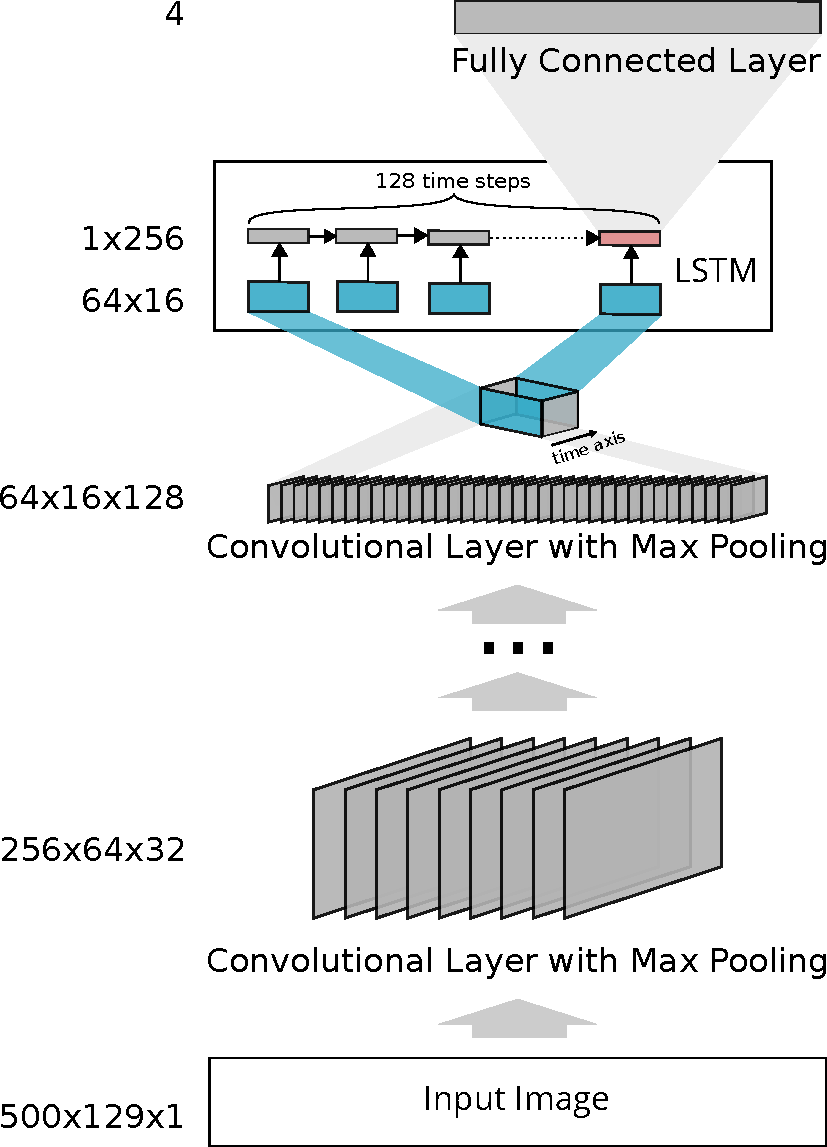
\includegraphics[width=\textwidth, keepaspectratio]{img/crnn.pdf}
    	\caption{Our proposed CRNN hybrid network architecture consists of two networks. A CNN transforms our input images into an intermediary representation of our audio frequencies. The 3D output of final convolutional layer of the CNN is sliced along the x-axis (time axis) into 2D time steps still containing all feature map information. The output of the final LSTM time step is fed into a fully connected layer for classification.}
    	\label{fig:crnn}
	\end{figure}
	
	\begin{figure}[]
  		\centering
    	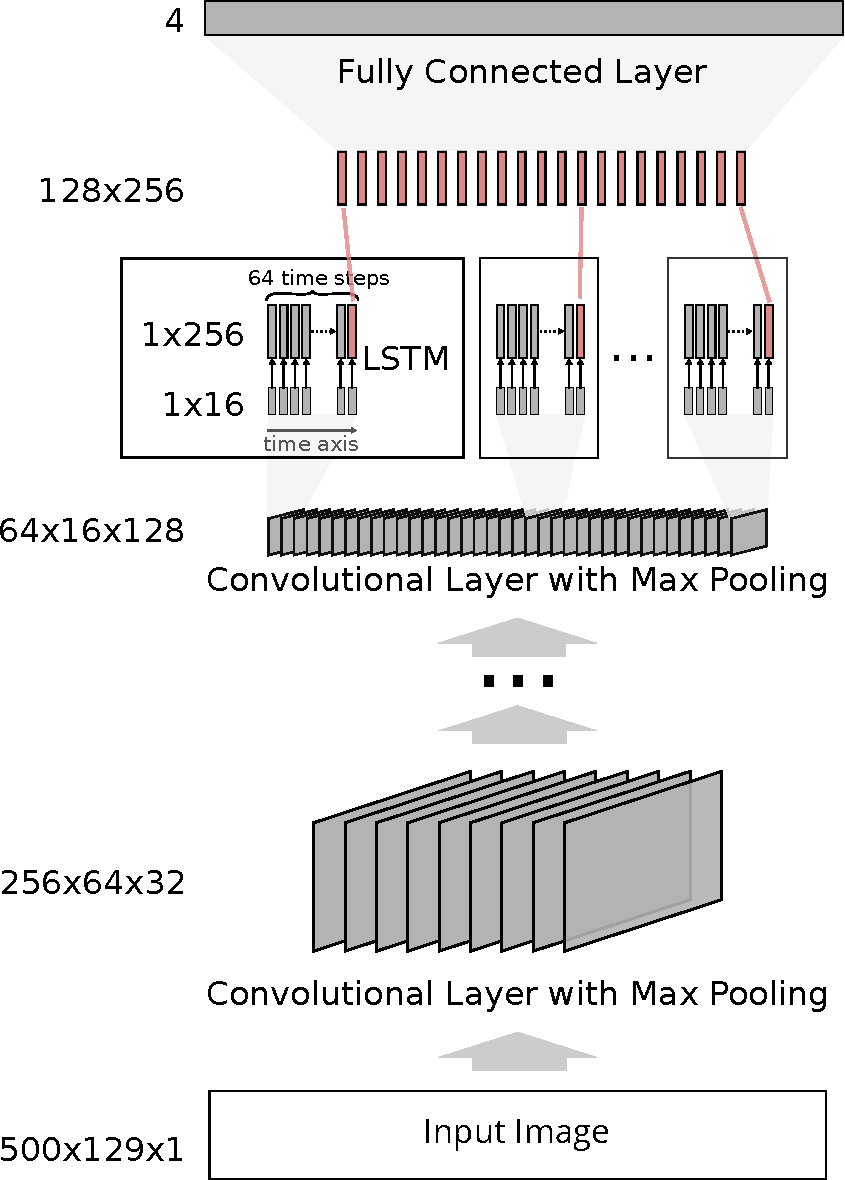
\includegraphics[width=\textwidth, keepaspectratio]{img/crnn2.pdf}
    	\caption{An alternative approach for a hybrid CRNN network. Each single feature map of the final convolutional layer is fed to separate LSTM networks as a 2D input. Each LSTM interprets the vector entries along the x-axis as time steps and operates on thin slice of the data. The output of the final time step of each LSTM is concatenated into a single vector serving as the input to a fully connected classification layer.}
    	\label{fig:crnn}
	\end{figure}

    \begin{itemize}
        \item Convolutional Recurrent Neural Networks
        \item What is their purpose? Averaging over predictions / fusion
    \end{itemize}

\subsection{Audio Representations}
\label{sec:audio_representations}
    \begin{itemize}
        \item MFCC
        \item Spectrogram
        \item Waveform
        \item Mel-scale
        \item frequency --> phoneme --> word --> sentence --> language
    \end{itemize}
    \section{Related Work}
\label{sec:related_work}

-wavenet?

Szegedy et al. reported several iterations of Google's convolutional neural network architecture, called GoogLeNet or Inception\cite{szegedy2015going, szegedy2016rethinking, szegedy2016inception}. These deep and very deep convolutional neural networks repeatedly set the state of the art record for minimal classification errors in the ImageNet Large Scale Visual Recognition Competition (ILSVRC). The presented network architectures present a number of advantages to previous CNN designs such as VGG. They introduced so called inception modules or mini networks that aim to factorize convolutions with larger filter size in order to accelerate training time and reduce the amount of model parameters. The idea is to replace larger spatial filter (e.g 5$\times$5 and 7$\times$7) which are disproportionally expensive in terms of computation with less expensive smaller inception modules with any loss of visual expressiveness. The inception modules are represented as a sequence of 3$\times$3 convolutions followed by a 1$\times$1 convolution. In case of 5$\times$5 filters they were able to achieve a gain of 28\% in computational speed up. The resulting Inception-v2 and Inception-v3 networks consist of 42 layers and are trained using the RMSProp\cite{tieleman2012lecture} optimizer. Compared to the VGG style networks they feature a lower overall computational cost while boosting better accuracy on image vision tasks.

A second innovation introduced by the inception networks is the use of a technique called batch normalization\cite{ioffe2015batch}. Training deep neural networks is complicated by the fact that the distribution of each layer's input changes during training, as the parameters of the previous layer change. This slows down trainings by requiring lower learning rates and careful parameter initialization. They refer to this phenomenon as internal covariate shift. The proposed solution to this problem is to normalize the inputs of each mini batch for the following layer. This results into a number of benefits. Foremost they were able to drastically reduce the time need to converge their models. Batch normalization enabled them to use higher learning rates without running into the vanishing or exploding gradient problem. Furthermore batch normalization acts as model regularizer positively affecting the generalization ability of the network. In turn this eliminates the need for dropout layers as regularizers. They conclude that simply by adding batch normalization to the convolutional layers of the inception network they were able to beat the state of the art of the ILSVRC challenge.



Shi et al.\cite{shi2016end} proposed an end-to-end trainable neural network for image-based sequence recognition and its application to scene text recognition. In their approach they used a hybrid neural network consisting of a convolutional part and a recurrent part for optical character recognition (OCR). They used convolutional layers as robust feature extractors for the input images and interpreted the resulting feature maps as a sequence of feature vectors. This sequence is fed into a LSTM network to capture the contextual information within the sequence. The whole CRNN was jointly trained with a connectionist temporal classification (CTC) loss \cite{graves2006connectionist} to output a sequence of letters. The found a VGG-based network architecture of seven convolutional layers with max pooling followed by a bidirectional LSTM to work best. They report that the use of batch normalization greatly accelerated their training time. Additionally they employed 1$\times$2 sized rectangular pooling windows instead of conventional squared ones. This tweak yielded feature maps of larger width and hence longer sequences for the RNN.

Song et al.\cite{song2015end} reported the use of an end-to-end trainable hybrid convolutional recurrent neural network for automatic speech recognition (ASR). They focussed on classifying a phoneme sequence of the input speech sample as part of an ASR system. Their proposed network consists of four convolutional layers, followed by two fully connected layers and is finalized by two LSTM layers. The network was jointly trained on the TIMIT dataset using CTC loss and used mel-filter bank greyscale images as input. Given the short length of the individual phonemes they operates on audio snippets of 15-25 milliseconds. Similarly to Shi et al. they resort to using rectangular pooling layers to obtain longer feature vector sequences. Their reported results are competitive to traditional gaussian mixture models and hidden markov models for ASR tasks. 

    \subsubsection{A UNIFIED DEEP NEURAL NETWORK FOR SPEAKER AND LANGUAGE RECOGNITION}
    \begin{itemize}
        \item \cite{richardson2015unified}
        \item Almost identical: Deep Neural Network Approaches to Speaker and Language Recognition \cite{richardson2015deep}
        \item high level overview of i-vector system
        \item Task: Language Recogniton + Speaker Recognition
        \item use bottleneck feature in the second to last layer
        \item input 7 static cepstra appended with 49 SDC
        \item DNN has 7 hidden layers of 1024 nodes each with the exception of the 6th bottleneck layer which has 64 nodes
        \item LRE11
    \end{itemize}
    
    \subsubsection{EXTRACTING DEEP NEURAL NETWORK BOTTLENECK FEATURES USING LOW-RANK MATRIX FACTORIZATION
    }
    \begin{itemize}
        \item \cite{zhang2014extracting}
        \item bottle neck feature improve classification results
        \item Task: Automatc Speech Recogniton (ASR)
        \item get bottleneck feature by low rank matrix factorization
        \item this is done by replacing the usual softmax layer weights by a linear layer with a small number of hidden units followed by a softmax layer
        \item BN laier is always last layer
        \item linear layer = FC without activation func
        \item uses DNN with 5 FCs with 1024 hidden units each + sigmoid activations + 1 BN layer
        \item softmax cross entropy loss 
        \item 23 critical-band energies are obtained from a Mel filter-bank, with conversation-side-based mean subtraction = 150 dimensions
        \item further reduciton of output by PCA
        \item hybrid system of DNN + BN feeding into DNN + BN
        
    \end{itemize}

\subsection{LRE 2015}

    \subsubsection{BAT System Description for NIST LRE 2015}
    \begin{itemize}
        \item \cite{plchot2016bat}
        \item participate in the "Fixed" and "Open" LRE Challenge
        \item segment data using automated Voice Activity Detection = previously trained NN
        \item 3042 segments (248 hours of speech) in train set and 42295 segments (146 hours of speech) in dev set.
        \item inputs 24 log Mel-scale filter bank outputs augmented with fundamental frequency features from 4 different f0 esti- mators
        \item used i-vector system
        
    \end{itemize}
    
    \subsubsection{Discriminating Languages in a Probabilistic Latent Subspace}
    \begin{itemize}
        \item \cite{sizovdiscriminating}
        \item Probabilistic Linear Discriminant Analysis (PLDA) model
        \item In this paper, we review state-of-the-art generative methods, based on the Total Variability (TV) model [10], with the aim to improve their performance with discriminative fine-tuning of each language cluster at a time.
        \item TV maps audio into single low-dimensional vector, i-vector, that contains speaker, channel, and phonetic variability
        
    \end{itemize}
    
    \subsubsection{Evaluation of an LSTM-RNN System in Different NIST Language Recognition Frameworks}
    \begin{itemize}
        \item \cite{zazo2016evaluation}
        \item used a one directional LSTM
        \item perform significantly better than i-vectors systems in LRE
        \item nice high level description of how LSTMs work
        \item inputs: random chunks of 2 seconds from which MFCC-SDC (Shifted Delta Coefficients) 
        \item softmax cross entropy loss
        \item use last frame for scoring
        \item comparison if i-vector baseline to LSTM
        \item only used training data for 8 languages with more than 200hours of data
        \item US English (eng), Span- ish (spa), Dari (dar), French (fre), Pashto (pas), Russian (rus), Urdu (urd), Chinese Mandarin (chi)
        \item data split into 3, 10 and 30 seconds
        \item model: two hidden layers of 512 units followed by an output layer. The hidden layers are uni-directional LSTM layers while the output layer is a softmax with as many units as languages in the cluster
        \item LSTM os only better for short utterance (<= 10s)
        \item LSTM uses less parameters than i-vector
        
    \end{itemize}
    
    \subsubsection{Frame-by-frame language identification in short utterances using deep neural networks}
    \begin{itemize}
        \item \cite{gonzalez2015frame}
        \item highlights the downsides/disadvantages of i-vector systems
        
    \end{itemize}
    
    
    
    
    \section{Datasets}
\label{sec:datasets}
	In this section we will explain the structure of our datasets, how we obtained them and what preprocessing steps are needed to extract our features.

	Recent breakthroughs in deep learning were fueled by the availability of large-scale, well-annotated, public datasets, for example ImageNet \cite{ILSVRC15}. Within the language identification community the TIMIT corpus of read speech \cite{garofolo1993darpa} has long been the default test set. TIMIT contains a total of 5.4 hours, consisting of 10 sentences spoken by each of 630 speakers from 8 major dialect regions of the United States recorded at 16kHz. Given the short span of each individual sound clip, the overall corpus duration and limitation to one language it was necessary to obtain our data from somewhere else. 
  
  	This thesis uses two primary datasets collected and processed by us. On the one hand we use speeches and statements from the European Parliament and on the other hand we rely on reports from news broadcasts sourced from YouTube.

\subsection{Language Selection}  

\subsection{EU Speech Repository}

	The EU Speech Repository is a collection of video ressources for interpretation students provided for free by the European Commission. The dataset is made up from debate of the European Parliament, commitee press conferences, interviews and tailor-made training material from EU interpretors. All audio clips are recorded in the speaker's native language and feature only one speaker.
	
		With 131 hours of speech data it is the smaller of the two datasets. We obtained material in four languages: English, German, French, and Spanish

\subsection{YouTube News Collection}

	Following the example of Montavon \cite{montavon2009deep} we looked for large, public sources of speech audio. We first experimented with podcasts and radio stations, both of which are unsuited for the job. Podcasts usually feature only one speaker and radio contains a lot of noise in the form of music. From these initial insights we noticed that news broadcasts provided high quality speech audio data. To source a large variety of languages and gather enough hours of speech audio we sourced the majority of our data from YouTube. 
	
	For each target language we manually selected one or more YouTube channels of respected news outlets. For example for English we used the BBC and CNN to gather a variety of different accents. For a full list of channels refer to table \ref{tab:channels}. All channels were chosen regardless of their content, their political views or journalistic agenda.
	
	\begin{table}[]
	\centering
	\begin{tabularx}{\textwidth}{ll}
	\toprule
	YouTube Channel Name  & Language \\ \midrule
	CNN                   & English \\
	BBCNews               & English \\
	VOAvideo              & English \\
	DeutscheWelle         & German \\
	Euronewsde            & German \\
	N24de                 & German \\
	France24              & French \\
	Antena3noticias       & Spanish \\
	RTVE                  & Spanish \\
	VOAChina              & Mandarin Chinese  \\
	Russia24TV            & Russian \\
	RTrussian             & Russian \\ \bottomrule
	\end{tabularx}
	\caption{YouTube Channel names and their corresponding language}
	\label{tab:channels}
	\end{table}

  	
  	Audio obtained from news coverage has many desired properties. The data is of high recording quality and hundreds of hours recording is available online. News anchors are trained to speak loud and clear, while still talking at a normal speed. News shows often feature guests or correspondents so we get a variety of speakers, which converse in a ordinary fashion with each other unlike speech audio obtained from reading texts aloud. Lastly, news shows feature all the noise one would expect from a real world situation: music jingles, non-speech audio from video clips and transitions between reports. The difficulty is also increased by mixed language reports. Many city, company, and personal names (e.g., New York City or Google for English) are pronounced in their native language and are embedded within the broadcast's host language. In essence we believe that speech data source from news broadcast represent an accurate, real-world sample for speech audio.
  	
  	In contrast to the EU Speech Repository this dataset consists 1024 hours of audio data for the same four languages: English, German, French and Spanish. We also gathered an extended language set adding Mandarin Chinese and Russian to the dataset. The extended set is only used for the evaluation of the model extensibility as outlined in section \ref{sec:extensibility}. Table \ref{tab:dataset_comparison} provides a complete comparison between the datasets.
  	
  	
\begin{table}[]
\centering
\begin{tabularx}{\textwidth}{lXXX}
\toprule
Feature               & EU Speech Repository & YouTube News & YouTube News \mbox{Extended} \\ 
\midrule
Languages             & English, German, French, Spanish & English, German, French, Spanish & English, German, French, Spanish, Russian, Chinese \\
Total audio duration  & 4                    & 4            & 6                     \\
Average clip duration & 4                    & 4            & 6                     \\
Audio Sampling Rate   & 4                    & 4            & 6                     \\ 
Training Samples      & 4                    & 4            & 6                     \\ 
\bottomrule
\end{tabularx}
\caption{Comparison of the EU Speech and YouTube News dataset}
\label{tab:dataset_comparison}
\end{table}
	



    \section{Implementation}
\label{sec:implementation}
This section outlines the software resources and frameworks used for implementing our language identification system. Given the datasets presented in Chapter~\ref{sec:datasets}, we describe the necessary data preprocessing steps to obtain the input audio representations for our network, as explained in Chapter~\ref{sec:theoretical_background}. Finally, we describe the concrete layer-wise model architecture of our CNNs and CRNN in detail.

\subsection{Software}
\label{sec:software}

	Our language identification system is implemented in Python~3 and uses the open-source deep learning framework Keras~\cite{chollet2015keras} with the TensorFlow backend~\cite{abadi2016tensorflow} for training our neural networks. Keras provides us with a set of higher-level machine learning primitives (such as convolutional layers) and optimization algorithms (including \emph{stochastic gradient descent}), without sacrificing any fine-grained control over the training parameters. Internally, Keras builds on Google's open-source numerical operation library TensorFlow, which is optimized for quickly computing multidimensional data on GPUs. We make heavy use Keras's aforementioned primitives, especially convolutional layers and the efficient LSTM implementation. Using the TensorFlow framework not only future-proofs our implementation but also enables us to readily deploy our model on mobile phones in the future.

	All models are stored on disk during training, including a summary of the layer architecture as well as the models' weights. This makes it easy to load, evaluate, and deploy all the models later. During the evaluation phase, all performance metrics (accuracy, precision, recall, F1 score) are calculated using the Scikit Learn framework~\cite{scikit-learn}. All measurements are logged and visualized using TensorBoard,\footnote{\url{https://www.tensorflow.org/how_tos/summaries_and_tensorboard/}, accessed 30 January 2017} both for the training and the validation set. Having the ability to easily study and compare different metrics such as accuracy and the loss value across several training runs made it very comfortable to continuously monitor the progress of our research. Figure~\ref{fig:tensorboard} shows a TensorBoard instance with plots of the metrics for several models.
%
	\begin{figure}[tp]
  		\centering
    	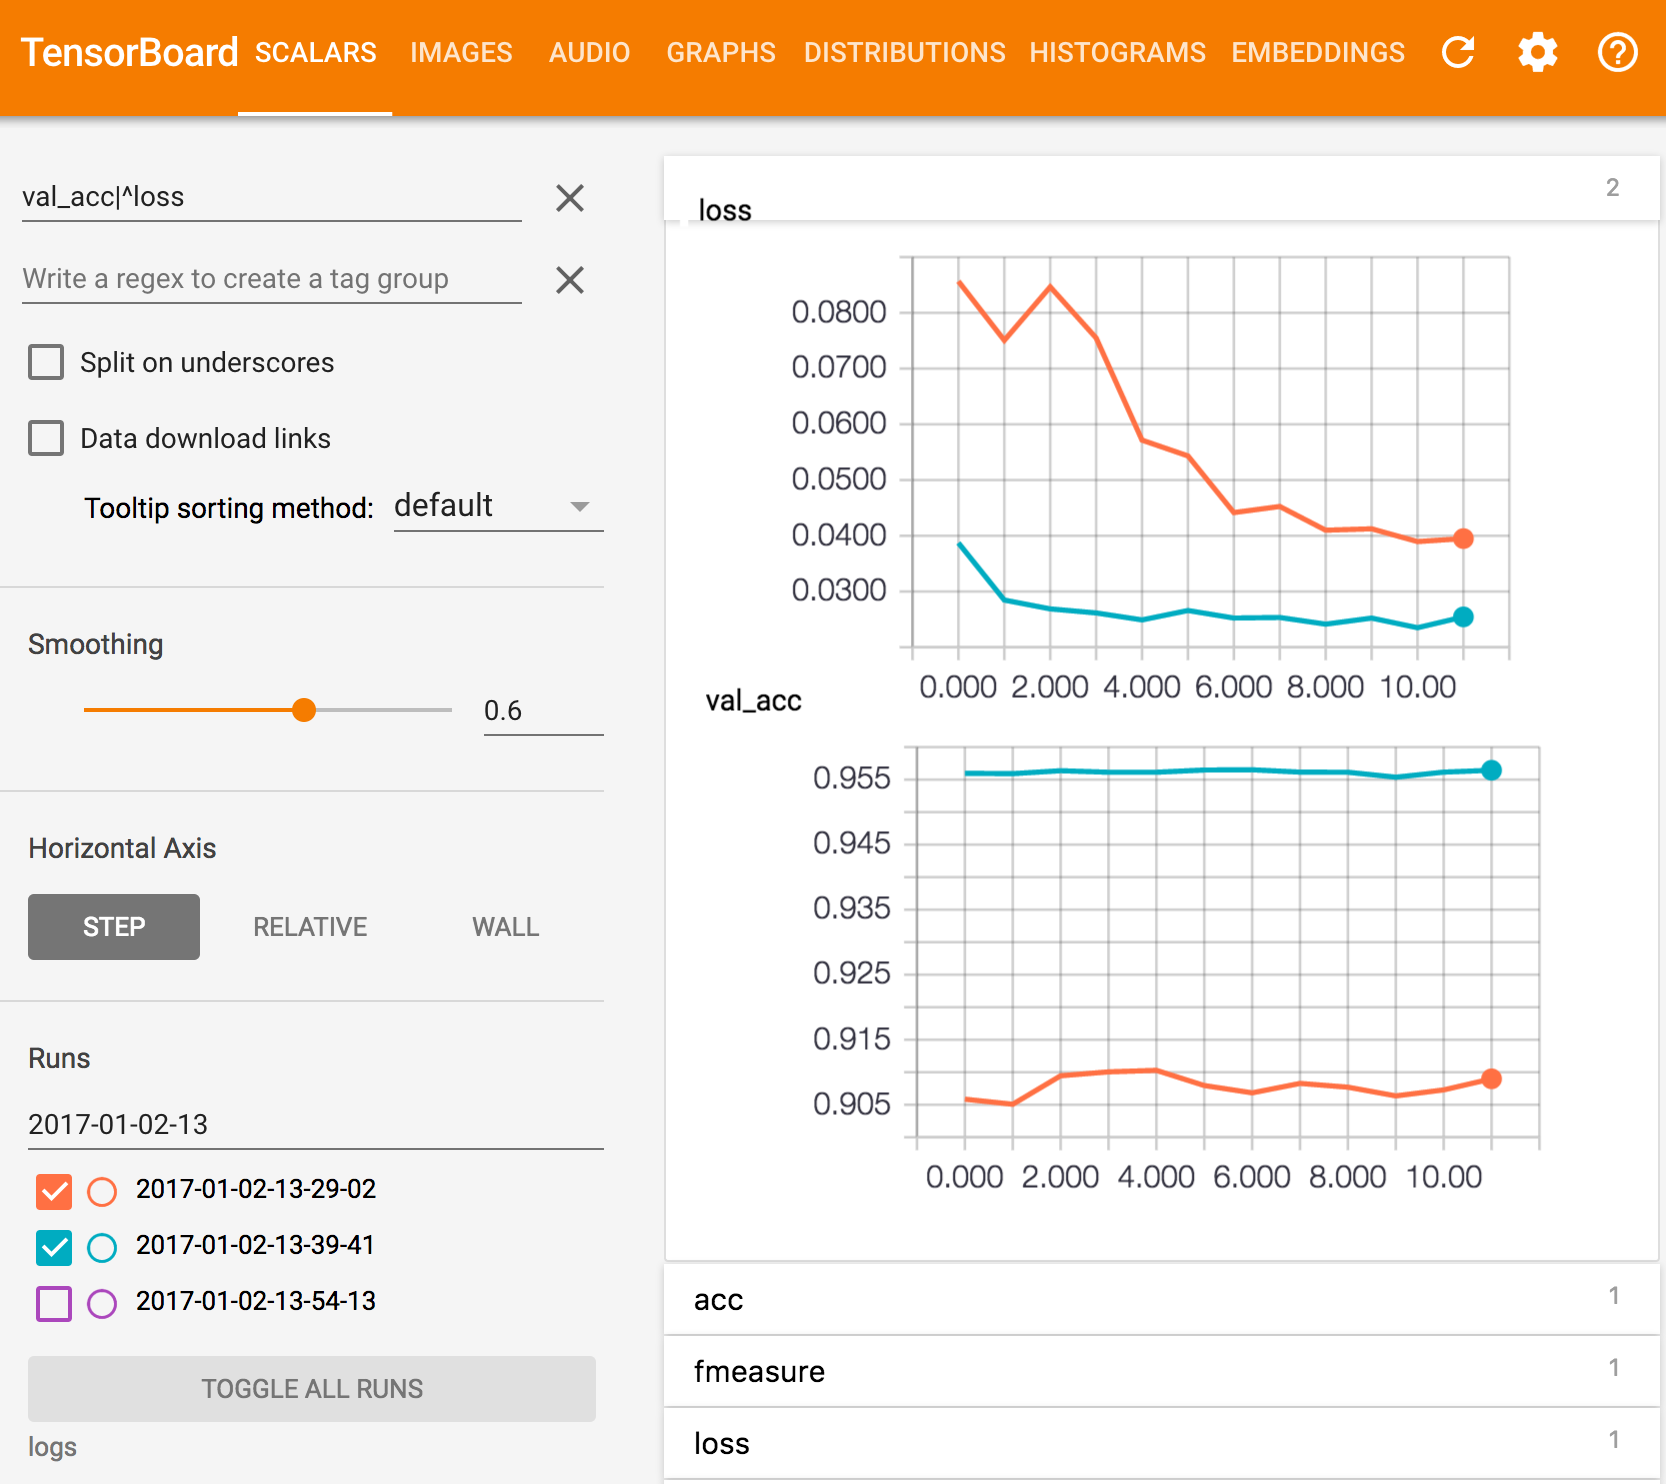
\includegraphics[width=\textwidth,keepaspectratio]{img/tensorboard2.png}
    	\caption{A TensorBoard instance showing training loss and validation accuracy of two different models. We regularly tried different approaches and model architectures and plotted multiple evaluation measures for comparison. This workflow enabled us to judge the impact of each experiment and measure the overall performance progress of the system.}
    	\label{fig:tensorboard}
	\end{figure}
%
We regularly compared different approaches and models against each other and used these plots to select the best performing systems for further experiments.

\subsection{Data Preprocessing}
\label{sec:data_processing}

	All audio files undergo preprocessing before being fed to the neural network. As a first step, all files are encoded in the uncompressed, lossless Waveform Audio File Format (WAVE\footnote{\url{http://www.microsoft.com/whdc/device/audio/multichaud.mspx}, accessed 23 February 2017}), commonly known by its file extension \texttt{*.wav}. This conversion has two advantages. First, a lossless data codec allows for future audio manipulations without any deterioration in signal quality and, second, makes the data easily interchangeable with third-party programs and libraries such as SciPy~\cite{scipy}.

	Since none our neural networks operate on raw waveform audio signals directly, we transfer our features into the image domain. As introduced in Section~\ref{sec:audio_representations}, we use a spectrogram representation of the audio data for training our models. The spectrograms are generated using the open-source command line tool SoX.\footnote{\url{http://sox.sourceforge.net/}, accessed 23 February 2017} The spectrograms are discretized using a Hann window~\cite{blackman1958measurement} and \num{129}~frequency bins along the frequency axis ($y$~axis), as instructed by the SoX manual.\footnote{\url{http://sox.sourceforge.net/sox.pdf}, p.~32, accessed 26 March 2017}
%
	\begin{figure}[tp]
  		\centering
    	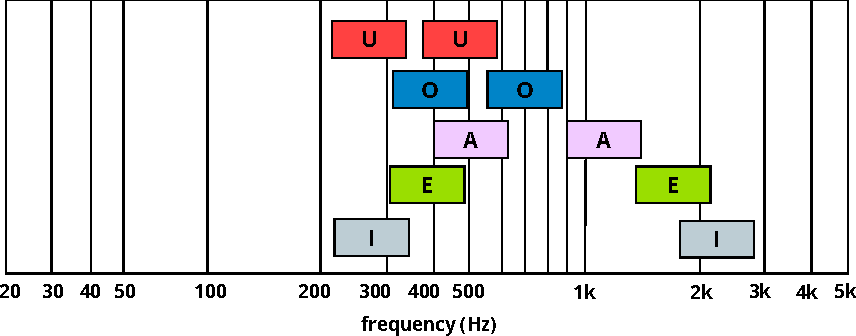
\includegraphics{img/frequencies.pdf}
    	\caption{The upper and lower frequency areas (\emph{formant}) for different vowels, typical for human speech. The lower speech formant $F_1$ has a total range of about \SI{300}{\hertz} to \SI{750}{\hertz} and the higher speech formant $F_2$ about \SI{900}{\hertz} up to over \SI{3000}{\hertz}. But each single spoken tone has a much narrower range for both formants.}
    	\label{img:frequencies}
	\end{figure}
%

	Male human voice frequencies begin between \SI{150}{\hertz}~and \SI{255}{\hertz}~\cite{traunmuller1993frequency}. Female voice frequencies are usually shifted by one octave and begin at~\SI{210}{\hertz}. Typically, voice frequencies range up to~\SI{3.4}{\kilo\hertz}. For reference, the human ear is capable of recognizing frequencies from \SI{20}{\hertz}~to \SI{20}{\kilo\hertz}, with most sensitivity in the region of between \SI{300}{\hertz}~and \SI{10}{\kilo\hertz}. Single sounds, however, exceed this limit significantly. Generally, voice frequencies are influenced by gender, age, as well as various other factors, such as the language, the type of discourse, and the emotional state of the speaker. Figure~\ref{img:frequencies} shows the frequency areas with high energy in response to the tone of different vowels of human speech for the English language.


Most phonemes in the English language do not exceed \SI{3000}{\hertz} in conversational speech.
Consequently, we instructed SoX to only include frequencies of up to~\SI{5}{\kilo\hertz} in the spectrograms.
The time axis ($x$~axis) is rendered at \num{25}~pixels per second. Each audio sequence is clipped into nonoverlapping ten-second segments. To avoid padding issues and segments shorter than ten seconds, the final segment is discarded. Since we gathered enough training data, we decided against padding with black pixels, which could be interpreted as silence and add unnaturally long speech pauses. We also decided against filtering silent sections within the ten-second audio segments to preserve the natural pauses between words and to not disturb the regular speech rhythm. 

	\begin{listing}[tp]
	\begin{lstlisting}[caption={SoX command and options used for generating monochrome spectrograms. All audio files were discretized into \num{129}~frequency buckets using a constant pixel width per time step, resulting in spectrogram images of $500 \times 129$ pixels.}, label={lst:spectrograms}]
sox -V0 input.wav -n remix 1 rate 10k spectrogram -y 129 -X 50 -m -r -o spectrogram.png

V0 - verbosity level 
n - apply filter/effect
remix - select audio channels
rate - limit sampling rate to 10k; caps max frequency at 5kHz according to Nyquist-Shannon sampling theorem
y - spectogram height
X - pixels per second for width
m - monochrome output
r - disable legend
o - output file
    \end{lstlisting}
    \end{listing}
    
Frequency intensities are mapped to an eight-bit grayscale range. We combined all audio channels into a single mono channel in order to generate only a single spectrogram image. The resulting grayscale images are saved as lossless, $500 \times 129$ PNG files. Listing~\ref{lst:spectrograms} shows the SoX command for generating a spectrogram image from an input audio file.


	As seen in Figure~\ref{fig:spectrogram}, the spectrograms feature very apparent bright ripple-like patterns.
%
	\begin{figure}[tp]
  		\centering
    	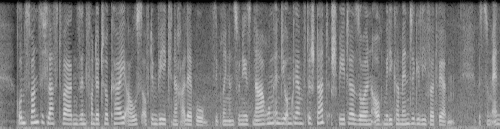
\includegraphics[width=\textwidth,keepaspectratio]{img/spectrogram.png}
    	\caption{A spectrogram generated from a German ten-second audio clip using SoX. Notice the bright ripple-like patterns representing intense frequency activations. We hypothesize that these frequency activations are suitable as the main features for the classifier.}
    	\label{fig:spectrogram}
	\end{figure}
%
	Each of these patterns represents a strong activation of a certain frequency at a point in time. Several frequency activations can be active simultaneously, constituting a particular phoneme or sound. A sequence of these phonemes forms words and is only interrupted by short speech pauses. We hypothesize that our \ac{lid} system learns the characteristical and unique composition of these frequency activations for every language in our classifier.

\subsection{Neural Network Architectures}
\label{sec:cnn_architecture}
To successfully solve our research task with deep neural networks, we have to design a fitting model architecture. Combing the right layers and adjusting the parameters correctly is not a trivial task. Critics argue that deep learning systems are a black box and that the impact of the individual layout of the network layers is hard to understand. Therefore, we base our model architectures on proven existing designs from related work and adapt them to our needs, while heeding best practices~\cite{mishkin2016systematic, szegedy2016rethinking}.

The architecture and the number of parameters of a deep neural network suited for a given task is determined by the bias--variance tradeoff~\cite{geman1992neural}. It is the goal of a network's author to avoid underfitting or overfitting the resulting model. Bias characterizes the prediction error that results from the model's limited ability to learn relevant relations between features in the training data. Underfitting can be caused by designing too small or too few network layers, causing a high bias. Variance, in contrast, refers to the error that results from the model responding overly sensitive to variation in the training data. Designing a too large network, introducing too many parameters, or adding too many layers result in a model with low variance. Hence, the model learns an exact representation of the training data without abstracting for more general applications. This is known as \emph{overfitting}.

Designing and adjusting the network layout is an iterative process. We tried many variations and parameters of our proposed model layouts to find the most suitable design for our LID system. The layout of the network interdepends and interacts with other design decisions of the system, especially the loss calculation. Each change in parameters involves a complete new training run to judge the effect of the change. Hence, the architecture always needs to be tested in its entirety.

In this thesis, we tried three different designs of convolutional neural networks. The first and second ones are based on the early VGGNet-like CNN-M model architectures by Simonyan et al.~\cite{Chatfield14}. The CNN features five convolutional layers and modest feature map output sizes. Note that the network's first two convolutional layers have comparatively large kernel size of $7 \times 7$ pixels and $5 \times 5$ pixels, respectively, yielding a large receptive field. Each convolutional layer is followed by batch normalization~\cite{ioffe2015batch}, a technique that helps in increasing training speed and achieving a higher level of model regularization. Following these layers, we added a $2 \times 2$ pooling layer with a stride of~\num{2}. After the five convolutional layers, we added regularization through a \SI{50}{\percent}~dropout before flattening all parameters to a fully-connected layer with \num{1024}~output units. The final, fully-connected layer serves as a classifier that outputs the language identification predictions. Henceforth, we refer to this model as CNN\_A. The full network layout can be seen in Table~\ref{tab:layers_CNN_A}.
%
 \begin{table}[tp]
  \centering
  \begin{tabu}{rcccc}
  \toprule
\textbf{Layer Type} & \multicolumn{2}{c}{\textbf{Output Size}} & \textbf{Kernel} & \textbf{Stride} \\
                          & \textbf{CNN\_A} & \textbf{CNN\_B} &             &     \\\midrule
Convolution               & 16     & 16   & $7 \times 7$  & 1   \\
Max Pooling               & 16     & 16   & $2 \times 2$  & 2   \\
Convolution               & 32     & 32   & $5 \times 5$  & 1   \\
Max Pooling               & 32     & 32   & $2 \times 2$  & 2   \\
Convolution               & 64     & 32   & $3 \times 3$  & 1   \\
Max Pooling               & 64     & 32   & $2 \times 2$  & 2   \\
Convolution               & 128    & 64   & $3 \times 3$  & 1   \\
Max Pooling               & 128    & 64   & $2 \times 2$  & 2   \\
Convolution               & 256    & 64   & $3 \times 3$  & 1   \\
Max Pooling               & 256    & 64   & $2 \times 2$  & 2   \\
Dropout \& Flatten        & 3328   & 832  &               &     \\
Fully-Connected           & 1024   & 256  &               &     \\
Fully-Connected           & 4      & 4    &               &     \\
  \bottomrule
  \end{tabu}
  \caption{The layerwise architecture for the convolutional neural networks CNN\_A and CNN\_B. These designs are based on early VGG-like networks and features large kernel size for the first two convolutional layers in an effort to capture a large receptive field of features.}
  \label{tab:layers_CNN_A}
 \end{table}

A slightly adapted version of CNN\_A has the same number of convolutional layers but features fewer feature maps. Instead of doubling the initial value of \num{16}~feature maps for every convolutional layer, we stick to a schedule of \num{16}--\num{32}--\num{32}--\num{64}--\num{64} feature maps, respectively. The fully-connected layer is also reduced to only \num{256}~output units. Overall, this model has significantly fewer parameters than CNN\_A. The purpose of this variation is to ensure that the architecture proposed for CNN\_A is not unnecessarily complex. We called this variation CNN\_B. The network layout of CNN\_B is also listed in Table~\ref{tab:layers_CNN_A}.

Lastly, we evaluate architecture CNN\_C, which is based on the VGGNet-16 network~\cite{simonyan2014very} and uses constant kernel size of $3 \times 3$ for all convolutional layers. At the same time, we increase the number of convolutional layers to seven and extend the number of feature map outputs for each layer to \num{64}--\num{128}--\num{256}--\num{256}--\num{512}--\num{512}--\num{512}. In CNN\_C, all fully-connected layers of are identical to CNN\_A. The main difference of this network design are smaller kernel sizes and, hence, a smaller receptive field of the convolutional layers. To compensate for this, we increase the number of layers. The complete CNN\_C architecture is laid out in Table~\ref{tab:layers_CNN_C}.
%
  \begin{table}[tp]
  \centering
  \begin{tabu}{rccc}
  \toprule
\textbf{Layer Type}              & \textbf{Output Size}  & \textbf{Kernel} & \textbf{Stride} \\ \midrule
Convolution             & 64     & $3 \times 3$    & $1 \times 1$  \\
Max Pooling             & 64     & $2 \times 2$    & $2 \times 2$  \\
Convolution             & 128    & $3 \times 3$    & $1 \times 1$  \\
Max Pooling             & 128    & $2 \times 2$    & $2 \times 2$  \\
Convolution             & 256    & $3 \times 3$    & $1 \times 1$  \\
Convolution             & 256    & $3 \times 3$    & $1 \times 1$  \\
Max Pooling             & 256    & $2 \times 2$    & $2 \times 2$  \\
Convolution             & 512    & $3 \times 3$    & $1 \times 1$  \\
Convolution             & 512    & $3 \times 3$    & $1 \times 1$  \\
Max Pooling             & 512    & $2 \times 2$    & $2 \times 2$  \\
Convolution             & 512    & $3 \times 3$    & $1 \times 1$  \\
Max Pooling             & 512    & $2 \times 2$    & $2 \times 2$  \\
Flatten                 & 6144   &                 &               \\
Fully-Connected         & 1024   &                 &               \\
Fully-Connected         & 4      &                 &               \\
  \bottomrule
  \end{tabu}
  \caption{The layerwise architecture for the convolutional neural network CNN\_C. With seven convolutional layers, this network design is deeper than the other two proposed CNN architectures. Additionally, the number of feature maps is increased to \num{512}~units compared to the \num{256}~units of the CNN\_A network. Overall, this network consists of a higher number of parameters than present in the other two designs.}
  \label{tab:layers_CNN_C}
 \end{table}


For our CRNN hybrid network, we construct a convolutional neural network followed by a recurrent neural network. Specifically, we use a bidirectional \emph{long short-term memory network} (\ac{lstm}) for the RNN part. We decided on using a bidirectional model of two LSTMs instead of a single LSTM based on the successful results of Shi et al.~\cite{shi2016end}. The CNN part of this network is tasked with extracting visual features and providing a high-dimensional intermediate frequency representation. The \ac{rnn} part splits the intermediate interpretation into a series of vectors (along the $x$ axis), which it treats as if they belonged to consecutive time steps.

In the CNN part, we repurpose the CNN\_A network architecture of five convolutional layers with larger kernels for the first two layers, since we found this CNN layout to work best for our LID task (details are provided later in Section~\ref{sec:results_news}). We also keep the batch normalization and max pooling layers. The bidirectional LSTM layer consist of two single LSTMs with \num{256}~output units each. We concatenate both outputs to a vector of \num{512}~dimensions and feed this into a fully-connected layer with \num{1024}~output units serving as the classifier. The complete model architecture can be seen in Table~\ref{tab:layers_CRNN}.
%
 \begin{table}[tp]
  \centering
  \begin{tabu}{rccc}
  \toprule
\textbf{Layer Type}       & \textbf{Output Size}    & \textbf{Kernel} & \textbf{Stride}  \\ \midrule
Convolution               & $123 \times 244 \times 16$  & $7 \times 7$    & $1 \times 1$    \\
Max Pooling               & $61 \times 122 \times 16$   & $2 \times 2$    & $2 \times 2$    \\
Convolution               & $57 \times 118 \times 32$   & $5 \times 5$    & $1 \times 1$    \\
Max Pooling               & $28 \times 59 \times 32$   & $2 \times 2$    & $2 \times 2$    \\
Convolution               & $26 \times 57 \times 64$   & $3 \times 3$    & $1 \times 1$    \\
Max Pooling               & $13 \times 28 \times 64$    & $2 \times 2$    & $2 \times 2$    \\
Convolution               & $11 \times 26 \times 128$   & $3 \times 3$    & $1 \times 1$    \\
Max Pooling               & $5 \times 25 \times 128$    & $2 \times 2$    & $2 \times 1$    \\
Convolution               & $3 \times 23 \times 256$    & $3 \times 3$    & $1 \times 1$    \\
Max Pooling               & $1 \times 22 \times 256$    & $2 \times 2$    & $2 \times 1$    \\
Transpose                 & $22 \times 1 \times 256$    &        &         \\
Reshape                   & $22 \times 256$           &        &         \\
Bidirectional LSTM & 1024                    &        &         \\
Fully-Connected    & 4                       &        &         \\
  \bottomrule
  \end{tabu}
  \caption{The layerwise architecture of the convolutional recurrent neural network. The network consists of two parts, a CNN and a bidirectional LSTM. This design shares its CNN architecture with the previously introduced CNN\_A. The final convolutional layer is sliced into time steps along the $x$ axis (time axis) and serves as input to LSTM.}
  \label{tab:layers_CRNN}
 \end{table}

We decided on training both parts of the hybrid network separately. First, we trained the CNN part by itself. This simplifies the task of learning the frequency features for the network. In practical terms, this means that we could reuse the model weights of the previously trained CNN\_A model. For the RNN part, we used a fine-tuning approach. This means that we froze all convolutional layers' weights by disallowing any further weight updates during the training phase. The bidirectional LSTM and \ac{fc} layers, however, remained unfrozen and continued to be subject to weight updates and were, hence, trained regularly. Later, we also experimented with unfrozen RNN weights, meaning that we trained and updated both the CNN and LSTM layers at the same time. This approach, however, yielded worse results, and we did not pursue it further.

    \section{Experiments and Evaluation} 
\label{sec:evaluation}
In this chapter we show and discuss the results of training the outlined neural network architecture for spoken language identification. We introduce several performance metrics and present the results evaluated on our system.
Further, we experiment with modified model architectures to optimize our model for noise robustness. To assess the real world performance of the the LID system we augment our data to simulated various noisy environments. We show the classification performance of our approach and discuss the system's inter language discrimination and extensibility to other languages.     

\subsection{Setup} 
\label{sec:setup}

\subsubsection{Hardware Resources}
\label{sec:hardware}
	In order to facilitate Keras' and TensorFlow's hardware-accelerated computation we executed all trainings on CUDA\footnote{\url{https://developer.nvidia.com/cuda-zone}, accessed 30.01.2017} compatible \ac{gpu} machines. All experiments were executed on two CUDA enabled machines belonging to the Internet Technologies and Systems chair. Details can be found in table \ref{tab:hardware}.
		
	\begin{table}[h]
	\centering
	\begin{tabularx}{\textwidth}{lll}
	\toprule
	  		& Machine A 					& Machine B \\ \midrule
	OS  	& Ubuntu Linux 14.04 		& Ubuntu Linux 16.04 \\
	CPU  	& Intel\textsuperscript{\textregistered} Core\textsuperscript{\texttrademark} i7-4790K @ 4GHz 	& AMD FX\textsuperscript{\texttrademark}-8370  @ 4GHz \\
	RAM  	& 16GB 						& 32GB \\
	GPU  	& Nvidia GeForce\textsuperscript{\textregistered} GTX 980 	& Nvidia Titan X \\
	VRAM  	& 4GB 						& 12GB \\
	\bottomrule
	\end{tabularx}
	\caption{Hardware resources used in training the neural networks.}
	\label{tab:hardware}
	\end{table}

\subsubsection{Data} 
\label{sec:data}
For our performance evaluation we used the European Speech Repository and YouTube News dataset as describe in section \ref{sec:datasets}. Both datasets were preprocessed and converted to spectrogram images as described in section \ref{sec:data_processing}. Each spectrogram image represents a non-overlapping ten second duration of source audio file. 
We split both dataset into a training (70\%), validation (20\%) and testing set (10\%) and all files were distributed equally between all four language classes. The number of samples per class were limited by the language with least files to ensure an equal class distribution. The European Speech repository yields a total of ca. 19.000 training images files which amounts to roughly 53 hours of speech audio. The YouTube News dataset is considerable larger and yields a total of ca .194.000 training files, or 540 hours. Table \ref{tab:data_splits} contains the detailed dataset splits.

	\begin{table}[]
	\centering
	\begin{tabularx}{\textwidth}{lrr}
	\toprule
	  				& European Speech Repository & YouTube News\\ \midrule
	Training Set    & 18.788						 & 193.432 \\
	Validation Set  & 5.372						 & 55.272 \\
	Test Set        & 2.684						 & 27.632 \\
	\midrule
	Total           & 26.844						 & 276.336 \\
	\bottomrule
	\end{tabularx}
	\caption{The amount of samples for our training (70\%), validation (20\%) and testing (10\%) set for the respective datasets.}
	\label{tab:data_splits}
	\end{table}

Given the European Speech Repository's smaller size we only used it initially confirm the validity of our approach. Since we were satisfied with the results we did not do include it in the extensive robustness tests that we used for the evaluation on the YouTube News dataset. In addition to the original audio we augmented the news dataset with three different background noises to evaluate how well our model would hold out in non ideal, real world situations outside of a new broadcasting studio. For the first experiment we added generic white noise to data. For the second experiment we added noise to simulate an old phone line or bad internet connection during voice chat. Lastly, we added background music to the data. All experiments are described in detail below.


\subsubsection{Training of the Neural Network Model} 
\label{sec:training}
Neural networks have a multitude of hyperparameters that influence the training results drastically. In this section we will briefly explain our choice of hyperparameters and other important training settings.

	\begin{description}
	\item[Optimizer] We employed an Adam\cite{kingma2014adam} optimizer to quickly and efficiently convergence our model. The Adam solver utilizes momentum during gradient updates to support a quicker convergence. We set the optimizer's parameters $\beta_1$ to 0.9, $\beta_2$ to 0.999, and $\epsilon$ to 1e-08. Overall we found it to be an order of magnitude quicker than using standard stochastic gradient descent (\ac{sgd}). We resorted to SGD during finetuning when we needed more control over the learning rate schedule and wanted smaller weight updates.
	\item[Weights Initializer] All layer weights are initialized within the range [0, 1) using Keras' default random Glorot uniform initializer\cite{glorot2010understanding}.
	\item[Data Normalization] The greyscale images are loaded using SciPy and normalized to the [0, 1] range. The shape for all inputs needs to be uniform across all samples and is set to [500, 129, 1], unless otherwise noted. The data loader uses Python generators\footnote{\url{https://docs.python.org/3/glossary.html#term-generator}, accessed 30.01.2017} to keep the system's memory footprint low.
	\item[Learning Rate] We set the initial learning rate to 0.001. Given the Adam optimizer's dynamic learning rate adaption we expect the learning rate to be increase or decreased after every epoch. 
	\item[Batch Size] We specified the batch size depending on the available VRAM of the training machine. We used a value of 64 for Machine A and 128 for Machine B. See section \ref{sec:hardware} for the hardware specifications. 
	\item[Weight Regularization] We employed the L2 norm as a weight regularizer for all convolutional and fully connected layers to improve the models generality. We penalize our loss with a weight decay value of 0.001. Additional regularization happens through the use of Batch Normalization layers.
	\item[Epochs] We limited the model training to a maximum of 50 epochs when using the Adam solver. We usually reach convergence well below this threshold. For training sessions with SGD we increased this parameter considerably. To speed up our workflow we employed an early stopping policy and stopped a training if the validation accuracy and loss did not increase within a ten epoch window.
	\item[Metrics] We observed the loss, accuracy, recall, precision, f1 measure, and equal error rate for both the training and validation set during model training. All values were saved to log files and visualized as graphs in TensorBoard.  
	\item[Loss] As is common for multivariate classification all models were trained with a softmax cross-entropy loss function.
	\end{description}


\subsection{Evaluation} 

\subsubsection{Evaluation Metrics} 
\label{sec:metrics}
In this section we discuss the evaluation metrics used throughout our experiments. All metrics are generally only defined for binary classification results. Given our multi-class classification problem we will report the average of the individual class performance measures in the following sections. 

\begin{description}
    \item[Accuracy] is a common measure in machine learning and is defined as the ratio of correctly classified samples to all samples in the dataset. In the context of language identification this translates as:
     
    	$$
		accuracy = \frac{\abs{\{\text{correctly identified language samples}\}}}{\abs{\{\text{all language samples}\}}}
		$$
     
    
    \item[Precision and Recall] Precision defines the ratio of retrieved language samples that are correctly identified as belonging to said language. Recall is the fraction of correctly identified language samples to all samples belonging to this language.
     
		$$
 		truePositives = \abs{\left\{\parbox{0.7\textwidth}{samples belonging to a language which were correctly identified as belonging to said language}\right\}} 
		$$
		
		$$
 		falsePositives = \abs{\left\{\parbox{0.7\textwidth}{samples belonging to a language which were identified as belonging to another language}\right\}}  
		$$
		
		$$
 		falseNegatives = \abs{\left\{\parbox{0.7\textwidth}{samples belonging to a language which were incorrectly identified as not belonging to said language}\right\}}  
		$$

	    $$
	    precision = \frac
	      {truePositives}
	      {truePositives + falsePositives}
	    $$
		
		$$
		recall = \frac
			{truePositives}
			{truePositives + falseNegatives}
		$$    


    \item[The F1 Score] is the scaled harmonic mean of precision and recall. It is used to a have combined judgement of recall and precision, since one is generally not interested in assessing one without the other.
    
    	$$
    	F1 = 2 * \frac{precision * recall}{precision + recall}
    	$$

\end{description}

\subsubsection{Results for EU Speech Repository Dataset}
\label{sec:results_eu}
In order to verify our theoretic model of using convolutional neural networks for classifying audio data in the image domain we established a baseline with the smaller EU Speech Repository dataset. Previous work with CNNs showed that the careful arrangement of the neural network layers has a great effect on the final classification performance. If one does not use enough or sufficiently large layers the model is not able to properly distinguish between classes. Going too deep or using too large layer outputs increases the overall number of model parameters to a degree where both training time and classification performance suffers again. The goal of this experiment is to find favorable settings for the number of convolutional layers needed, the kernel size of the convolutions, the number of output maps of the convolutional layers and finally the number of features of the fully connected layer.

For this particular dataset we tested three slightly different model architectures. Following the VGG-style model architecture of Simonyan et al. \cite{Chatfield14}, we setup a first CNN with five convolutional layers as outlined in section \ref{sec:cnn_architecture}. The first two convolutional layers use larger kernel sizes of 7x7 and 5x5, respectively. All following kernels were set at 3x3. Each convolutional layer is followed by batch normalization and a 2x2 pooling with a stride of two. After the five convolutional blocks we add regularization through a fifty percent dropout before flattening all parameters to a fully connected layer with 1024 outputs. The final fully connected layer serves as a classifier outputting the prediction for our language identification. Henceforth, we will refer to this model as CNN\_A.

A slightly adapted version called CNN\_B has the same amount of convolutional layers but with a reduced number of feature maps. Instead of doubling the initial value of sixteen feature maps for every convolutional layer we stick to a schedule of 16 - 32 - 32 - 64 - 64 feature maps, respectively. The fully connected layer has also been reduce to only 256 output units. Overall this model has significantly less parameters than the CNN\_A. The purpose of this variation is to ensure that the proposed architecture for CNN\_A is not unnecessarily complex.
	
Lastly we evaluated architecture CNN\_C which uses constant kernel size of 3x3 for all convolutional layers. At the same time we increased the number of convolutional layers to seven and extended feature maps for each layer: 64 - 128 - 256 -256 - 512 - 512 - 515. The remaining fully connected layers are identical to the CNN\_A. The main difference here is the smaller receptive field of the convolutional layer which could negatively effect the model performance but should speed up the model training time overall. The complete CNN\_C architecture is laid out in table \ref{tab:layers_CNN_C}.

	\begin{figure}[]
  		\centering
    	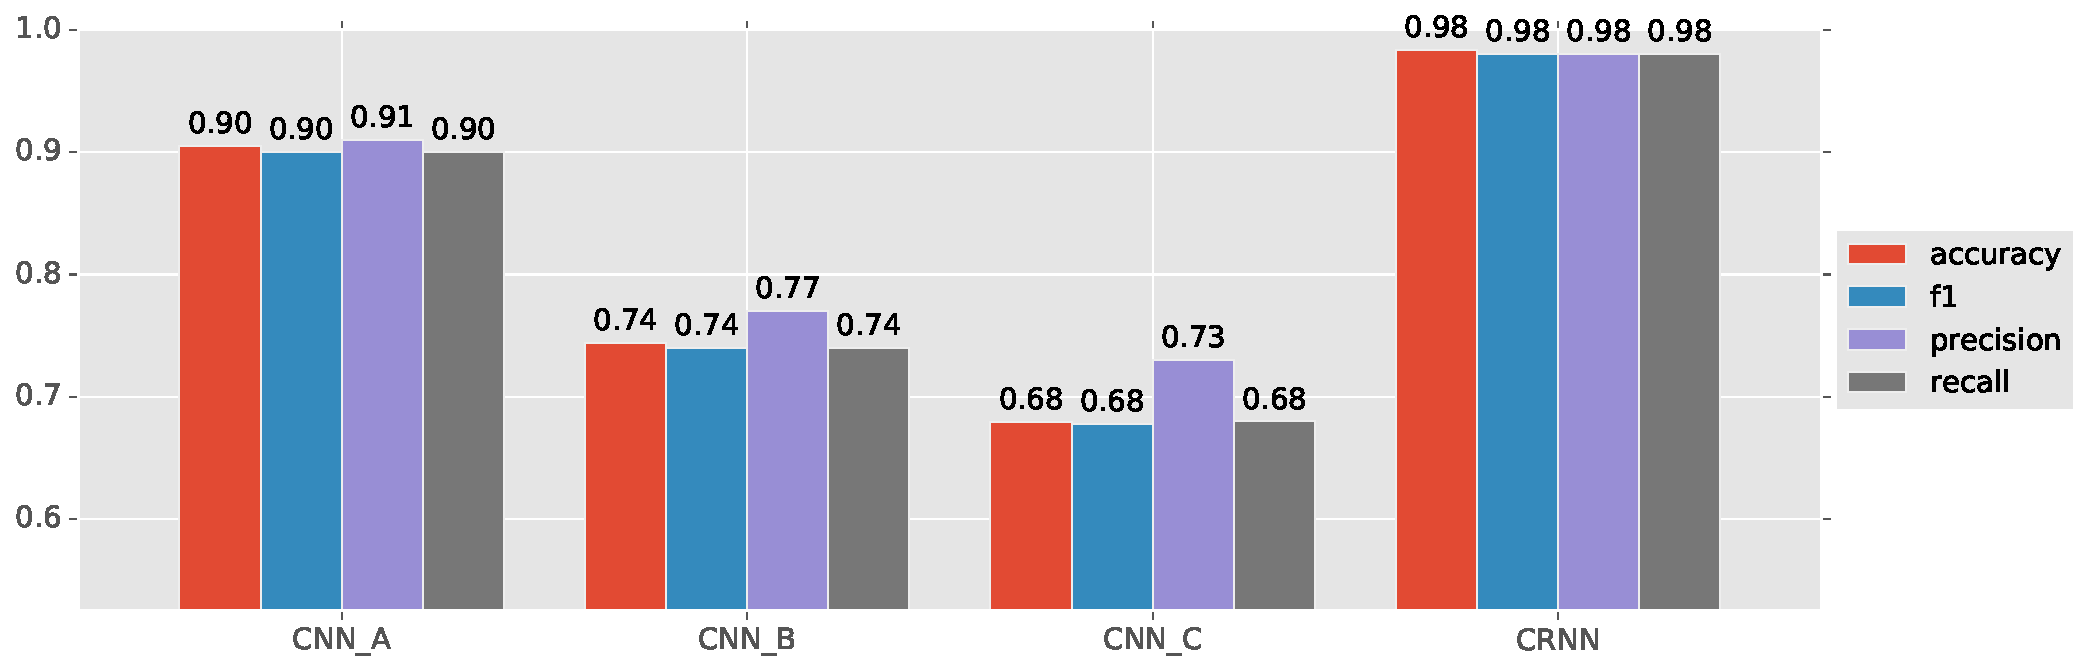
\includegraphics[width=\textwidth, keepaspectratio]{plots/results_eu_plot.pdf}
    	\caption{Performance measure comparison of three different CNN architectures evaluated on the EU Speech Repository dataset and our proposal of a \ac{crnn} model. CNN\_A outperforms all other CNN approaches with a top accuracy of 0.90, but is bested by the CRNN's 0.98 accuracy, proving the potential of this thesis' approach.}
    	\label{fig:eu_results}
	\end{figure}

CNN\_A outperforms both of the other two network architectures with respect to all the evaluated performance measures, cf. figure \ref{fig:eu_results}. With a top-1 accuracy of 0.904 it trumps CNN\_B and CNN\_C with 0.743 and 0.68, respectively. Comparing the F1 score we get a similar result: 0.90 versus 0.74 and 0.68. This experiment confirmed a few of our initial hypotheses. Firstly, it proves that convolutional neural networks can be successfully used to classify audio data. Secondly, it demonstrates that spectrogram images are meaningful representation for audio that retains enough information for language identification. Thirdly, it shows that large kernels for the initial convolutional layers are indeed favorable. The increased receptive field captures both the time domain and frequencies better. 
Based on these findings we did some further testing with CNN\_A. Based on Mishkin et al.\cite{mishkin2016systematic} we switched the convolutional layers' ReLU activations to Exponential Linear Units\cite{clevert2015fast} (ELU) but without any improvement. Baoguan et al. \cite{shi2016end} proposed to use 1x2 rectangular pooling windows instead of the conventional square ones. This tweak yields feature maps with larger width, hence longer features along the time domain. In theory this should increase the CNN's sensitivity at judging the occurrence of frequencies at certain time intervals. For this experiment we were unable to gain any improvement, but we will discuss this approach some more for our CRNN approach later.

The goal of this thesis is to evaluate the use of Deep Convolutional Recurrent Networks. Therefore we extended our previously best performing CNN\_A with a bidirectional \ac{lstm} layer. We interpreted the \ac{cnn} output as intermediate representation of the audio frequencies and used every vector entry along the x-axis as a single step / input for the LSTMs as explained in section \ref{sec:hybrid_networks}. During the training we froze the convolutional layers to only train the LSTMs weights and learn the frequency sequence of the audio sample. Our bidirectional LSTM layer trained two individual LSTMs with 512 outputs each, one training the input sequence from the start and one from the end. Both outputs were concatenated to form a single output vector with 1024 dimensions which is followed by single fully connected layer for classification.
Our CRNN architecture outperformed all CNN approaches significantly. With a top-1 accuracy of 0.98 and a F1 score of 0.98 it proves the viability of the CRNN approach and reaffirms the central hypothesis of this thesis.


\subsubsection{Effect of Audio Duration} 
\label{sec:duration}
For all previous experiments we split all audio recording into ten second segments, which translated into an image dimension of 500x129 pixels for the spectrogram. We decided on 10 second audio snippets based on the setup of the \ac{nist} LRE 2015 \footnote{\url{https://www.nist.gov/itl/iad/mig/2015-language-recognition-evaluation}, accessed 15.02.2017} challenge. To study the effect of the audio duration on classification performance we set up a version of the EU Speech Repository dataset with non-overlapping five seconds snippets but left the number of frequency bins unchanged. Hence we reduced the input dimensions to 250x129 pixels and could not just use our previously trained models but had to retrain new models.

To set a baseline we used the same CNN\_A architecture as explained in the previous section. When completely training it from scratch we achieved an accuracy of 0.81 falling short of the results achieved with ten second snippets. Next, we applied some transfer learning and finetuned CNN\_A on the new five second dataset. Since the convolutional layers are not bound to a specific input size and given that the frequency features did not change in dimension we were able to reuse the complete  convolutional weights. For the finetuning we froze the convolutional layers, confident in their ability to detect frequencies, and only retrained the final two fully connected layers. With the bisection of the input data the amount of model parameters were greatly reduced, especially the fully connected layer weights. To account for this we finetuned one model with a fully connected layer of 512 outputs and a second one with the default 1024 outputs. Overall this yielded an accuracy of 0.88 and 0.89, respectively. We concluded that the effect of the smaller fully connected layer is only marginal. 

After establishing a solid CNN foundation we applied the same CRNN approach as previously highlighted. Due to the shorter audio duration the final pooling layer only features 5 output units along the x-axis compared to the 13 output units of the ten second CRNN. When interpreted as a sequence of time steps and fed into the bidirectional LSTM the accuracy improved only marginally to 0.90. We suspect that the number of time steps was too little to take full advantage of the recurrent network layer.
In an effort to increase the number of output units of the final pooling layer and hence increase the sequence length we applied 1x2 rectangular pooling tweak again. We changed the final two pooling layers and bumped up the number of output units along the x-axis to 22. The y-axis remained unaffected. The resulting accuracy of 0.90 and the F1 score of 0.91 remained comparable to the previous model and did not bring the desired effect. 

In summary we believe that decreasing the duration of the audio snippets used for training has a negative effect on the classification performance. While it is possible to train and finetune CNNs that match their ten second counterparts we found that the CRNN approach does not boost the model effectiveness in a similar manner.
	
	\begin{table}[]
	\centering
	\begin{tabularx}{\textwidth}{lrr}
	\toprule
	Model Architecture		& Accuracy 		& F1 	\\ \midrule
	CNN from scratch    		& 0.81			& 0.81 	\\
	CNN finetuned (\ac{fc} 1024)	& 0.88			& 0.89 	\\
	CNN finetuned (FC 512)	& 0.89			& 0.89 	\\
	CRNN with 5 time steps	& 0.90			& 0.91 	\\
	CRNN with 22 time steps & 0.90			& 0.91 	\\ \midrule
	CRNN (10s) for reference& 0.98			& 0.98 	\\ 
 	\bottomrule
	\end{tabularx}
	\caption{Various CNN and CRNN model configurations trained on five second audio samples. The best performing five second CRNN still falls short of its ten second counterpart with an accuracy of 0.90 and 0.98, respectively.}
	\label{tab:audio_duration}
	\end{table}


\subsubsection{Results for YouTube News Dataset}
\label{sec:results_news}
Following the promising results from the experiments with the EU Speech Repository we switched to the ten time larger YouTube News dataset for further training and evaluation.
For our first experiment we used the same CNN\_A architecture as before but initialized the model weights with the weights of best performing model of the EU Speech Repository evaluation. Our reasoning here was to reuse the convolutional layers that were already trained to identify frequency ranges. However, with an accuracy of only 0.79 it did not perform as strongly as anticipated. One reason for this could be that the EU dataset is a lot smaller and does not feature as many diverse situation as present in news broadcasts since all audio is recorded in a similar environment without much background noise and exhibits high signal quality.

Next, we trained the same CNN completely from scratch with randomly initialized weights. We had several setbacks when using an Adam optimizer and reverted to using standard SGD to keep our loss in check. Additionally we employed gradient clipping to avoid the exploding gradient problem. With these measure we were able to get the model to converge and gained an accuracy of 0.9090 besting our previous attempt. 
Given the new dataset larger size we also tried to increase the number of parameters by doubling the feature maps of the convolutional layers. This, however, did not help.
As a next step we applied the CRNN approach again. Based on this CNN we added our bidirectional LSTM layers in the same manner as for the previous CRNNs and were able to slightly improve our accuracy and F1 score to 0.9124, respectively. 

To evaluate how our model architecture fares against established deep learning models we trained a model using Google's Inception-v3\cite{szegedy2016rethinking} layout. This resulted in a top accuracy of 0.9488 improving our results significantly. Applying the established CRNN treatment to this model increased the performance by roughly 1\% to an accuracy of 0.9579. In order to boost the performance even further we also tried a CRNN variation where both the convolutional layer weights and the LSTM weights were trained. In contrast to our initial CRNN approach this method also updates the existing convolutional filter. We found, however, that this variation did not improve performance.
Figure \ref{fig:news_results} shows an overview of the performance metrics of the mentioned experiments.
The increased performance, however, does not come without a cost. With a total of 3.153.924 parameters our CRNN uses roughly six times less parameters then the Inception-v3 CRNN with its 19 million. This increases training time, requires more training data and consumes more GPU memory. On disk the serialized model weights come in at 30MB versus 260MB, which could be a potential disadvantage for deployment on mobile phones.

	\begin{figure}[]
  		\centering
    	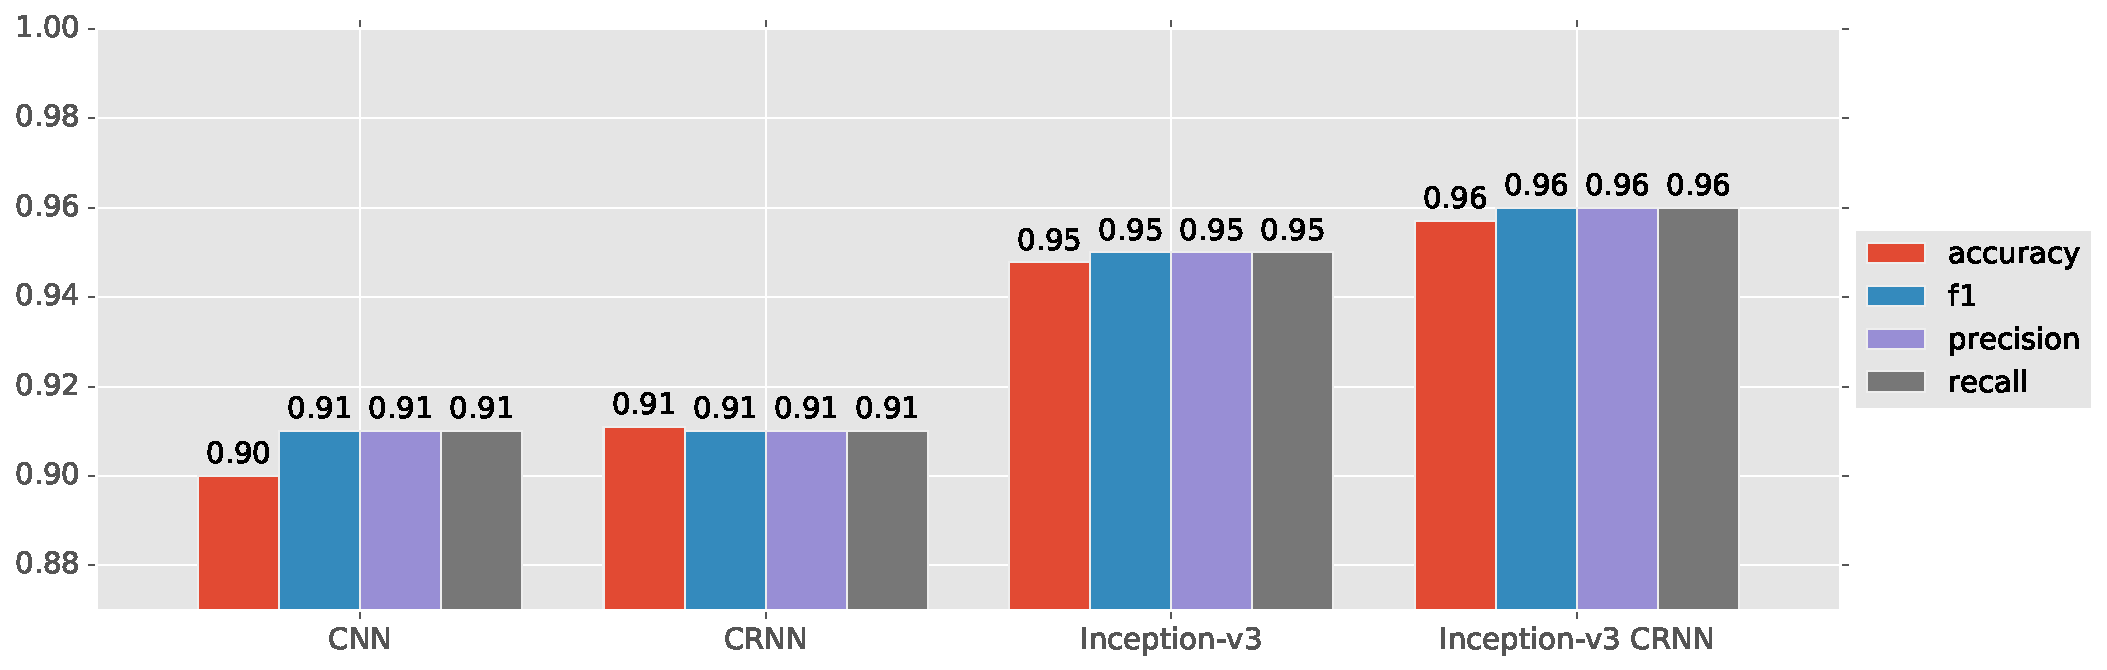
\includegraphics[width=\textwidth, keepaspectratio]{plots/results_news_plot.pdf}
    	\caption{Performance measurement comparison between our CNN and CRNN models and Inception-v3 based models. With a top accuracy of 0.96 the Inception style CRNN performs best but needs more than five times the amount of parameters compared to our proposed model architecture.}
    	\label{fig:news_results}
	\end{figure}
	
	\todo{Plot trainings loss as a space filler?}


\subsubsection{Inter Language Discrimination} 
\label{sec:lang_discrimination}

Previous work\cite{montavon2009deep} raised concerns about the similarity of our four feature languages \textendash{} English, German, French and Spanish \textendash{} and the model's inability to discriminate between them properly. Both English and German belong to the West Germanic language family, while French and Spanish are part of the Romance languages. We hypothesized that our deep learning approach to language identification is able to differentiate between them reliably. 
Table \ref{tab:language_family_crnn} shows the confusion matrix when evaluating language family pairs on the best performing CRNN. Spanish and French audio files separate very well with hardly any wrong classifications. Both languages are more likely to be classified as German and English rather then as the respective other, demonstrating that their learned representations are quite distinctive within their language family. 
German and English language samples have a tendency to be misclassified as the respective other. Furthermore English also has a slight bias towards French, an observation in line with related work\cite{werkmeister2016practical}. German, however, distributes its classification error evenly between French and Spanish. Overall, German samples are misclassified the most across all languages.

	
	\begin{table}[]
	\centering
	\begin{tabularx}{\textwidth}{l|rrrr}
	      & EN     & DE     & FR     & ES \\ \midrule
	  EN  & 6153   & 339    & 181    & 225 \\
	  DE  & 426    & 6128   & 173    & 162 \\
	  FR  & 200    & 145    & 6447   & 107 \\
	  ES  & 214    & 170    & 115    & 6399 \\
	\end{tabularx}
	\caption{Confusion matrix of the best performing CRNN. English audio files are likely to be misclassified as German and vice versa. Both languages belong the family of Germanic languages. }
	\label{tab:language_family_crnn}
	\end{table}

	The confusion matrix for the Inception-v3 CRNN, table \ref{tab:language_family_inception}, match our observations for the other model. Again, German exhibits the most classification errors. 
	
	\begin{table}[]
	\centering
	\begin{tabularx}{\textwidth}{l|rrrr}
	      & EN     & DE     & FR     & ES \\ \midrule
	  EN  & 6648   & 140    & 45     & 61 \\
	  DE  & 152    & 6639   & 62     & 44 \\
	  FR  & 68     & 59     & 6742   & 27 \\
	  ES  & 75     & 83     & 42     & 6697 \\
	\end{tabularx}
	\caption{Confusion matrix of the Inception-v3 CRNN. Despite its deeper architecture it makes the same mistakes as our proposed CRNN. }
	\label{tab:language_family_inception}
	\end{table}
 

\subsubsection{Noise Robustness} 
\label{sec:noise_robustness}
Given that we left our data unadulterated we expect a certain degree of noise within the dataset. Therefore we hypothesize that the neural network develops some noise robustness by itself. For instance, the convolution operations of the earlier layers summarize pixel values over an image patch and help with masking noise. To prove our theory we generated two augmented datasets based on the YouTube news dataset. 
For the first one we mixed the audio signal with randomly generated white noise sound. The resulting audio samples are still easily identifiable for human listeners. The noise has a very strong audible presence, so much so that a human tester will easily be annoyed after a few seconds of listening to it.
For the second augmentation we added a more periodic cracking noise emulating analog telephony or a bad voice chat connection. We sampled a selection of fitting sound effects and randomly applied these to the source signal using the PyDub\footnote{\url{https://github.com/jiaaro/pydub}, accessed 01.03.2017} library. The resulting noise is not as noticeable and less intrusive as the white noise, but gives the augmented audio file a subdued vintage quality.

The white noise did deteriorate the language identification performance significantly both for our CRNN proposal and the Inception-v3 CRNN as can be seen in table \ref{tab:noise}. The noise spectrogram in figure \ref{fig:noise} show that the white noise effect has a very strong influence on the resulting image. Most parts of the image end up being covered by the distinct noise texture and only the lower frequency features remain intact. All pauses and fine grained details are lost to the noise sound. 
The cracking experiment fared did not incur such a dramatic drop in performance. That might be in part due to the consistent recurring sound of the noise in contrast to the randomly generated white noise sound. Perhaps a second factor was the lower, less intrusive volume used for augmenting this dataset.

The deeper, more complex structure of the Inception-v3 CRNN did suffer a significantly smaller performance deterioration than our proposed CRNN model architecture. The more than five times as many parameters seem to capture the frequency features in a more robust manner. In an attempt to remedy the performance loss for our model we trained and finetuned models containing white noise data. We experimented with a 100\% noise dataset and the original news dataset extended with 10\% white noise for augmentation purposes. While both approaches did recovered some white noise performance they reduced the general language identification and cracking noise statistics as a trade off.
Let it be noted that our audio mixing was fully automated and that the resulting samples varied in speech and noise volume. We tried to match volume levels of speech and noise to maintain as much clarity of speech as possible, yet some samples will have an artificial quality to them.

	\begin{figure}[]
  		\centering
    	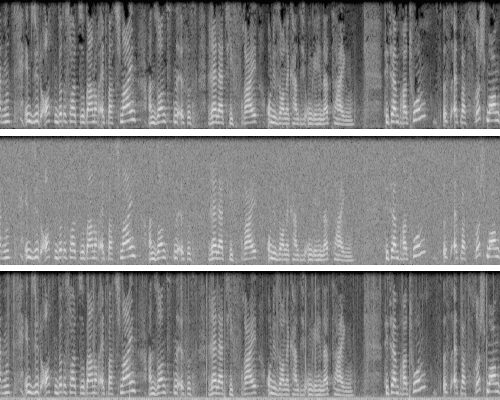
\includegraphics[width=\textwidth, keepaspectratio]{img/noise_spectrograms.png}
    	\caption{Spectrograms generated from the raw data, augmented with white noise and mixed with a cracking noise emulating analog telephony or a bad voice chat connection. The white noise aggressively subdues most higher frequencies and pauses causing a loss of classification performance. The cracking noise is less intrusive and therefore does not affect accuracy as much.}
    	\label{fig:noise}
	\end{figure}


Overall we note that even deep convolutional recurrent networks are still subject to the influence of noise on audio. We learned that our spectrogram preprocessing does not help in these situations and that different network architectures play an instrumental role in dealing with these situations.
 
	\begin{table}[]
	\centering
	\begin{tabularx}{\textwidth}{lrrrrr}
	\toprule
	Dataset & \multicolumn{2}{c}{CRNN} & \multicolumn{2}{c}{Inception-v3 CRNN} \\  
                & Accuracy  & F1    & Accuracy  & F1   \\ \midrule
white noise     & 0.63      & 0.63  & 0.91      & 0.91 \\
cracking noise  & 0.82      & 0.83  & 0.93      & 0.93 \\
 	\bottomrule
	\end{tabularx}
	\caption{Accuracy and F1 score for our models evaluated on the speech data augmented with two different types of noise.}
	\label{tab:noise}
	\end{table}



\subsubsection{Background Music Robustness} 
\label{sec:music_robustness}
Many real world audio applications involve a some form of music. Therefore we evaluated our model to see if language identification was still possible when mixing speech with music. For this experiment we used two different test sets. For the first series we augmented our existing YouTube news dataset with randomly sampled background music in a similar fashion to the background noise augmentation. The background audio was obtained from Soundcloud\footnote{\url{https://soundcloud.com/royalty-free-audio-loops}, accessed 01.03.2017} and features royalty free, instrument-only music from various genres, including Pop, Dubstep, Rock and Electro amongst others. 
We normalized the volume of these sounds and overlaid them onto our speech data while trying to stay below the speech audio volume. In the best cases the two audio streams blend nicely with the background music producing a soft but noticeable ambient effect, while retaining the clarity of the speech. In other cases the audio levels and volume are over-accentuate for one or the other. The final result, however, does neither resemble a song nor a piece of music. We changed neither the tempo nor the pitch of our speakers and the rhythm of the vocals does not match the rhythm of the background audio. Therefore we gathered a small second test set of XXX \todo{insert number of songs} songs for each of the following genres: Pop, Rock, Hiphop, and Folk. 
Given that our training set does not intentionally include samples with music or songs we expected the performance do be drastically lower then for pure speech samples.

	\begin{table}[]
	\centering
	\begin{tabularx}{\textwidth}{lrrrr}
	\toprule
Dataset & \multicolumn{2}{c}{CRNN} & \multicolumn{2}{c}{Inception-v3 CRNN} \\   
                  & Accuracy  & F1    & Accuracy   & F1   \\ \midrule
Background Music  & 0.70      & 0.70  & 0.89  & 0.89 \\
Pop Songs         & 0.XX      & 0.XX  & 0.XX  & 0.XX \\
Rock Songs        & 0.XX      & 0.XX  & 0.XX  & 0.XX \\
HipHop Songs      & 0.XX      & 0.XX  & 0.XX  & 0.XX \\
Folk Songs        & 0.XX      & 0.XX  & 0.XX  & 0.XX \\

 	\bottomrule
	\end{tabularx}
	\caption{Accuracy and F1 score for our models evaluated on the speech data augmented with background music and songs sampled from four different genres.}
	\label{tab:audio_duration}
	\end{table}

\subsubsection{Model Extensibility} 
\label{sec:extensibility}
So far all our experiments were conducted on datasets consisting of only four languages: English, German, French and Spanish. We complemented these with two new languages spoken by millions around the globe: Mandarin Chinese and Russian. The goal of this experiment was to learn whether we could easily expand our model to other languages. 
We increased our existing YouTube news dataset with samples taken from Chinese and Russian news channels yielding the extended YouTube news dataset described in section \ref{sec:youtube_news}. In order to maintain the class distribution for six languages we had to decrease the number of training samples of the existing samples slightly. Table \ref{tab:dataset_comparison} contains the details for the extended YouTube news dataset.

For this experiment we first finetuned our previous best CNN by replacing the final fully connected layers and adjusted the number of output nodes to accommodate for six classes. The resulting model served as the basis for training the CRNN in a similar manner as in earlier experiments. Applied on the test set we measured an accuracy of 0.92 and F1-score of 0.92. Both measurements match our previous evaluation with four languages on the YouTube news dataset as laid out in section \ref{sec:results_news} proving that the proposed CRNN architecture can easily be extended to cover more languages. Figure \ref{fig:6lang} shows individual performance measure of each language. Mandarin Chinese outperforms all other languages with a top accuracy of 0.96, which could be interpreted as it sounding the most contrasting to western languages and featuring its own unique intonation. We also noted that Russian was most frequently misclassified as Spanish and vice-versa. In contrast to our previous observation German is no longer the worst performing class, but English takes that role now. This is in part due to a significant number of misclassification as Russian samples.

	\begin{table}[]
	\centering
	\begin{tabularx}{\textwidth}{lrrrr}
	\toprule
     & accuracy & precision & recall  & F1   \\ \midrule
EN   & 0.86     & 0.89      & 0.88    & 0.88 \\
DE   & 0.89     & 0.91      & 0.90    & 0.90 \\
FR   & 0.93     & 0.94      & 0.93    & 0.94 \\
ES   & 0.92     & 0.91      & 0.93    & 0.92 \\
CN   & 0.96     & 0.97      & 0.96    & 0.96 \\
RUS  & 0.92     & 0.90      & 0.92    & 0.91 \\

 	\bottomrule
	\end{tabularx}
	\caption{}
	\label{tab:6lang}
	\end{table}
	\todo{Include the table or is the plot enough?}

	\begin{figure}[]
  		\centering
    	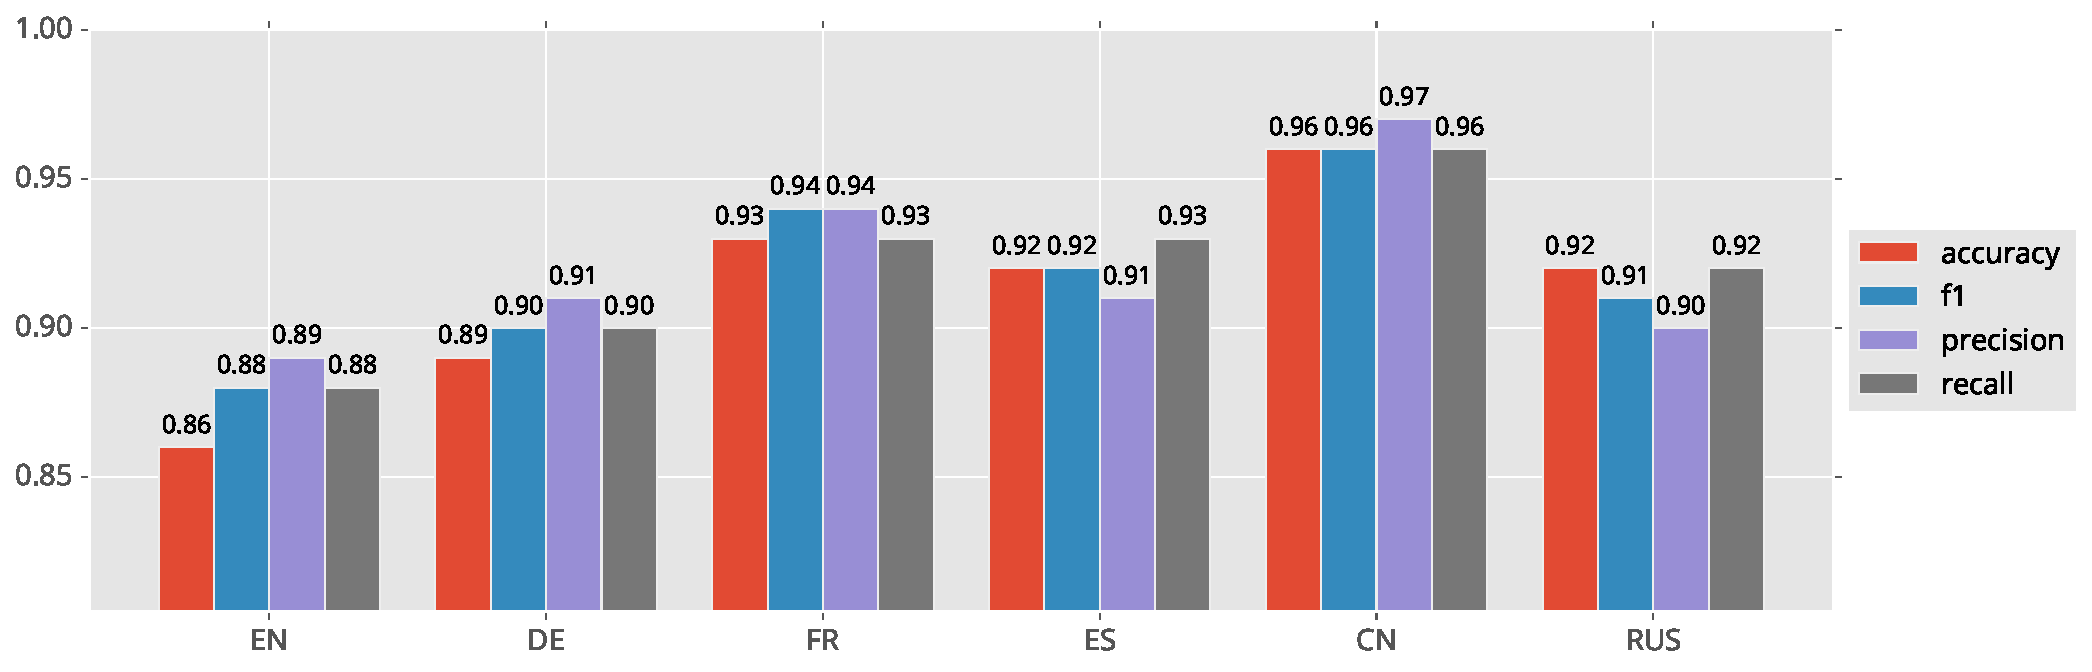
\includegraphics[width=\textwidth, keepaspectratio]{plots/results_6lang_plot.pdf}
    	\caption{Individual performance measurements for each of our six target languages: English, German, French, Spanish, Mandarin Chinese, and Russian. Chinese exhibits the lowest misclassification rate while English performs the worst. Overall the model performance is consistent with previous evaluations on four languages as highlighted in section \ref{sec:results_news}.}
    	\label{fig:6lang}
	\end{figure}

Given that both new languages are rooted within their own respective language families and feature considerable different intonations we were content to find that the features learned by our model are indeed universal in nature. We are confident in the believe that the approach to language identification proposed in this thesis can be successfully applied to a wide variety of languages.

\subsubsection{Visualizations} 
\label{sec:visualization}
All previous sections described and evaluated our model by measuring various performance indicators and applying them to different datasets. In this section we will present plots underlining earlier observations from a different perspective.

	\begin{figure}[h]
  		\centering
    	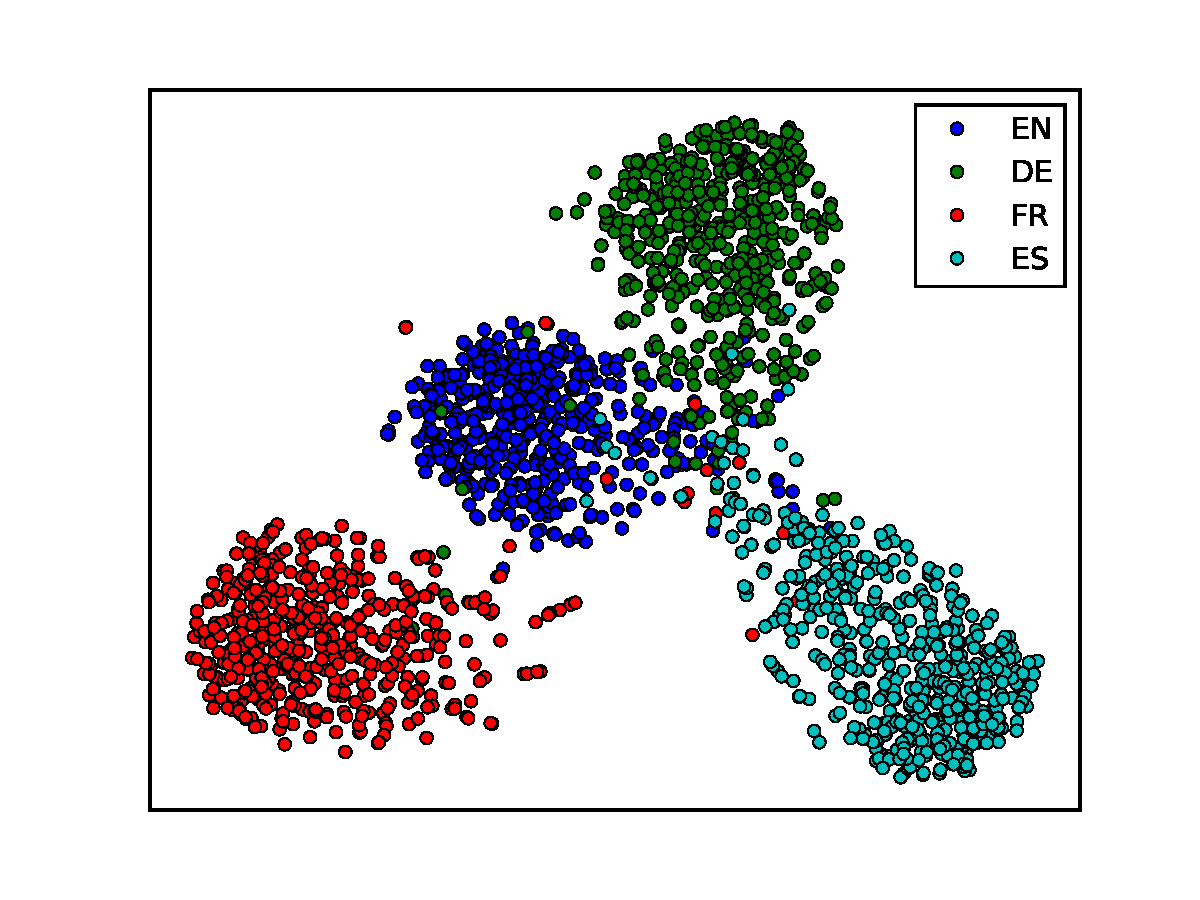
\includegraphics[width=\textwidth, keepaspectratio]{plots/tsne.pdf}
    	\caption{A 2D t-SNE plot of the high dimensional vector representation of our YouTube news samples. All four language classes form distinct clusters confirming the network learned effective representations of the audio features.}
    	\label{fig:tsne}
	\end{figure}

First we visualized the high dimensional language vector embedding space using the  t-distributed stochastic neighbor embedding (\ac{tsne}) algorithm\cite{maaten2008visualizing}. t-SNE is a nonlinear dimensionality reduction technique employed to map high dimensional data into 2D or 3D space for plotting. We applied this machine learning algorithm to the first 2000 predictions of our second to last fully connected layer right before the classifier and managed to project our 1024 dimensional YouTube news data into a 2D space. Figure \ref{fig:tsne} shows the resulting plot highlighting a good separation of our four language classes as independent clusters confirming the network learned effective representations of the audio features. Note that French and Spanish split very nicely while German and English have some overlap. This is in line with our previous observations of classification errors as described in section \ref{sec:youtube_news}.

A primary advantage of deep neural networks is their ability to identify and learn useful features on their own making them powerful and versatile. From an end user's perspective they can appear as a bit of a black box and it remains unclear which features they ultimately deem relevant. In order to get a better understanding of our model we visualized its convolutional layers. In figure \ref{fig:conv_filter} we visualized nine of the highest activating filters of the final convolutional layer. In order to obtain these filters we performed back propagation from the output of the filter back to an input image. This yielded the gradients of the output of the filter with respect to the input image pixels. We used that to perform gradient ascent, searching for the image pixels that maximize the output of the filter.

Visualizations for the lower level convolutional layers resulted in images of very simple geometric shapes like lines and circles which matched our expectations. With increasing network depth each convolutional layer's features combined and evolved into more complex shapes resembling our input domain. In figure \ref{fig:conv_filter} we can identify the familiar ripple like patterns that form frequency activations over time. This proves that the network learned these structures as we hypothesized earlier. We can also identify that some filters specialize in high frequency whereas others focus on low frequencies. Furthermore, it can be observed that the filters only react to a short and specific span of time within the spectrogram, all of which are less than one second in duration.

	\begin{figure}[h]
  		\centering
    	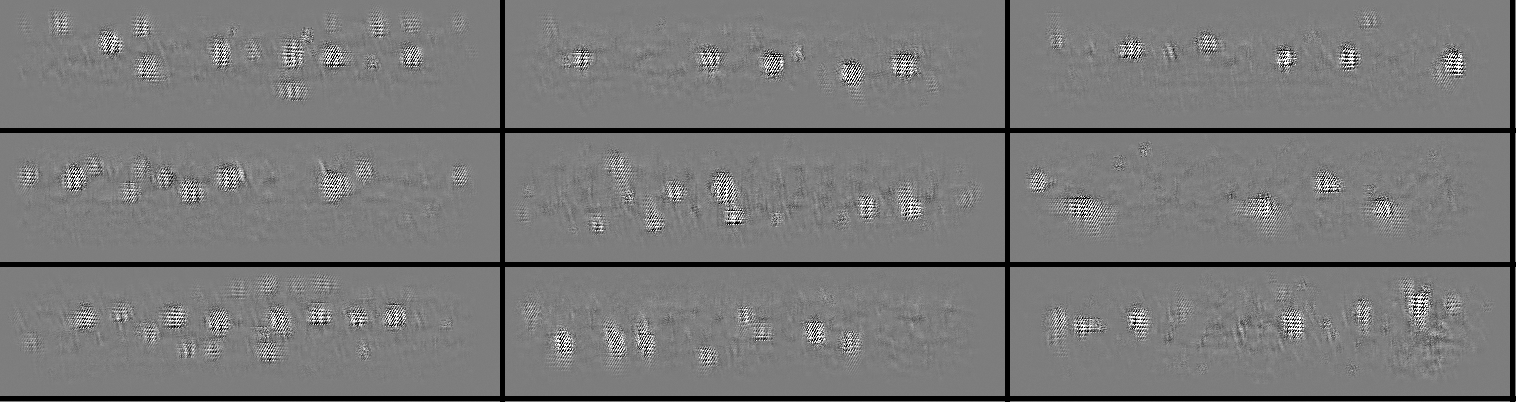
\includegraphics[width=\textwidth, keepaspectratio]{img/conv_filter.png}
    	\caption{Visualization of nine filters of the final convolutional layer. Note the ripple like patterns responsible for detecting different frequency spans in the input audio.}
    	\label{fig:conv_filter}
	\end{figure}

\subsubsection{Discussion} 
\label{sec:comparison}
In this section we introduced and compared different CNN and CRNN architectures for language identification and proved that these models can be used to accurately solve our research task. We showed that these results hold true regardless of the input audio source and across various languages. This thesis also confirms that audio tasks can be solved within the image domain using spectrogram image representations. As hypothesized we were able to prove that our system learned the audio and frequency structures of these spectrogram images. We demonstrated that the learned intermediate language representations were indeed universal and not language specific and could easily be applied to other languages as well.
 Our approach of combining convolutional neural networks with bidirectional long short term memory cells showed a consistent improvement over baseline CNNs. In general we were able boost accuracy by at least 1\%. Furthermore, we established that an Inception-v3 style CRNN outperformed all other approaches both in terms of accuracy (0.96) as well as with noise robustness. 

We presented several augmented datasets to evaluate both noise and background music robustness. We were content to note that the noise resistance of the Inception-v3 CRNN reached acceptable levels without us having to modify or restructure our algorithm. This reaffirms our believe in deep learning techniques as a viable tool for audio tasks.

Our CRNN approach interpreted every vector entry along the x-axis as a separate time step for the recurrent layer. Hence, all results gathered here are representative of only ten seconds of an audio file. We believe that in a production ready system we could increase the performance by doing a majority voting across multiple segments of a longer audio file.

\todo{Anything else here???}


    \section{Conclusions and Future Work}
\label{sec:summary}
This last chapter presents high-level insights and finally comments on
future work and prospects concerning the discussed topics.
This chapter further outlines the contributions of this thesis and concludes the work done
in the research field.

\subsection{Future Work}
The overall trend within the deep learning community over the past few years was to increase the network depth by adding more and more layers. Supporting this development, however, is becoming increasingly difficult. Very deep networks are harder to train and require ever more computing time. One way to gain higher accuracy scores is to change the design and architecture of the network. He et al. recently proposed the technique of \emph{deep residual learning} to tackle these challenges~\cite{he2016deep}. In their network architecture, the authors introduce small building blocks of two convolutional layers, in which the second layer receives the original input of the first layer in addition to the output of its predecessor~\cite{he2016deep}. Using this approach, the authors were able to train the so-called ResNet with \num{152}~layers and bested the previous state of the art in the ILSVRC 2015 challenge. Similarly, Szegedy et al. introduced the latest iteration of their Inception networks using these residual connections as well~\cite{szegedy2016inception}.

For future work, we think that using deep residual neural network for the convolutional part of our architecture holds much promise. In this thesis, we were able to measure our best results using the previously state-of-the-art \emph{Inception-v3} network for computer vision tasks. In the future, we believe that using Inception-v3 or the ResNet architecture should improve our results even further and, perhaps, add more robustness to noise as well.

As part of our training process, we pretrained our convolutional neural networks before assembling them to the complete CRNN. The complete CRNN then reused the learned weights of the convolutional layers and fine-tuned them by a further, joint training step with the LSTM part. This \emph{transfer learning} approach is fairly simple yet effective. Unfortunately, in parallel to fine-tuning the network on the new data, the CRNN starts to forget previously learned features. This is referred to as \emph{catastrophic forgetting}. Rusu et al. introduced \emph{Progressive Neural Networks} as a novel approach to \emph{transfer training}~\cite{rusu2016progressive}. This technique leverages prior knowledge via so-called \emph{lateral connections} to previously learned features. For future work, we think that it is worthwhile to evaluate whether this approach could be helpful in improving our transfer learning steps.

We formulated our research problem as a classification problem for language identification. The limitation of this is, however, that our models are only able to accurately predict languages that were part of the training corpus. In other words, we are unable to identify any language unknown to the system. An interesting, yet slightly different research field, is metric learning. This approach is able to measure a difference or a score between its classes. For example, with metric learning, a sample would receive a score indicating whether it was more closely related to either German or English. The advantage of this approach is that the system is no longer limited to only the training languages. For unknown languages, one could still assess whether a language is more similar to one than another. Conversely, this also allows for judging how different an input is to any language known to the system, something that is not possible with our approach.

In this thesis, we evaluated our networks on six different input languages. In the future, our system could be extended to cover even more languages. In our work, we did not evaluate the effectiveness of the presented approach on similar tasks such as dialect identification. Future work could evaluate the accuracy of our approach on the fine-grained differences between dialects and accents of a language.

Throughout this work, we evaluated our models' robustness to white noise and background music noise. We also tried evaluating our models on songs but found the performance to be inadequate for our needs. In our case, the biggest problem with songs was the fact that the speech frequencies are completely masked by the frequencies of the instruments. Future work could focus on language identification for songs and music.

Our approach relies on extracting and classifying a sequence of intermediate language representations created from spectrogram image inputs. Within the automatic speech recognition community (ASR), there is related work on extracting and classifying sequences of phonemes~\cite{song2015end}. Instead of matching these phoneme sequences to words, one could use these to classify a target language. This is an alternative approach to the one presented in this thesis and could be used to compare the effectiveness and robustness of the two methods. Another interesting idea was introduced by Google's \emph{Wavenet}~\cite{van2016wavenet}. By utilizing dilated convolutions for speech recognition, the authors were able to capture a longer receptive field, which is much cheaper to compute than LSTMs. Further, \emph{Wavenet} operates on raw audio signals forgoing the need for spectrogram features.  Even though \emph{Wavenet} was evaluated for automatic speech recognition, it could likely be adopted to language identification as well. 

\subsection{Conclusions}
In this thesis, we presented several neural network architectures aimed at the task of solving the language identification problem. We employed CNNs and CRNNs to infer the language of given audio samples directly from their spectrogram representation. 

We proposed three hypotheses and conducted experiments to verify their validity. We confirmed that, first, convolutional neural networks are an effective, high-accuracy solution for language identification tasks. Second, spectrogram images are a suitable input representation for learning audio features. Third, convolutional recurrent neural networks consistently improve the classification accuracy throughout all experiments compared to a plain, CNN-based approach.

We presented and discussed the availability and suitability of various datasets for LID. For our research, we compiled and processed more than a thousand hours of speech data from public sources---one the one hand, speeches and press conferences from the European Parliament, and on the other hand, audio from news broadcasts hosted on YouTube.

To judge the effectiveness and validity of our research in several scenarios, we augmented our test dataset with additional white noise, crackling noise, and background music and tested the robustness of our neural networks. We reported a decrease in recognition accuracy under these noisy situations.

In this work, we explored different neural network architectures and commented on our setup of hyperparameters. Our best-performing CRNN model is based on the Inception-v3 architecture and was able to achieve an accuracy and F1~score of~\num{0.96} and~\num{0.96}, respectively.

Initially, we trained and evaluated our models on four languages---English, German, French, and Spanish. We were content to find that the approach presented in this thesis could be transferred to other languages as well. During our experiments, we added Mandarin, Chinese, and Russian. The frequency features learned by our system are, indeed, language-independent, and we were able to expand our system to these two new languages without any large modifications.

This thesis presents a recent approach to solve the language identification task with deep neural networks. Further research needs to be deducted to improve the robustness against noise and to discover new kinds of layers and architectures to support even higher accuracies in this field. 

    \begin{appendices}
\section{Audio manipulation with SoX}

    \begin{lstlisting}[caption=Generating monochrome spectrograms with SoX]
    sox -V0 input.wav -n remix 1 rate 10k spectrogram -y 129 -X 50 -m -r -o spectrogram.png
    
    
    
    V0 - verbosity level 
    n - apply filter/effect
    remix - select audio channels
    rate - limit sampling rate to 10k; caps max frequency at 5kHz according to Nyquist-Shannon sampling theorem
    y - spectogram height
    X - pixels per second for width
    m - monochrome output
    r - disable legend
    o - output file
    \end{lstlisting}
    
    \begin{lstlisting}[caption=Adding white noise to an audio file]
    scale_factor1=0.94; 
    scale_factor2=0.05;
     
    sox -m \
        -v $(echo "$(sox input.wav -n stat -v 2>&1) * ${scale_factor1}" | bc -l)  input.wav \
        -v ${scale_factor2} <(sox input.wav -p synth whitenoise) \
        -b 16 output.wav
   \end{lstlisting}

\end{appendices}

    % Inhaltsverzeichnis
    \clearpage % auf neuer Seite
    \bibliography{referenzen}

\end{document}
